% LTeX: language=pt-GB

\documentclass{book}

\usepackage{titlesec}
\usepackage{fourier-orns}


\usepackage[utf8]{inputenc}
\usepackage[T1]{fontenc}
\usepackage{lmodern}
\usepackage[margin=1in]{geometry}
\usepackage{amsmath,amssymb,amsthm,mathtools}
\usepackage{graphicx}
\usepackage{tikz-cd}
\usepackage{bbm}
\usepackage{stmaryrd}
\usepackage{enumitem}
\usepackage{algorithm}
\usepackage{algpseudocode}
\usepackage{mdframed}
\usepackage{microtype}

\usepackage[table]{xcolor}
\usepackage{array}
\usepackage{booktabs}


\usepackage{tcolorbox}
\usepackage{pgfplots}
\usepackage{booktabs}
\usepackage{array}
\usepackage{tikz}
\pgfplotsset{compat=1.18}

\renewcommand{\arraystretch}{1.8}
\setlength{\tabcolsep}{14pt}



\usepackage{fancyhdr}
\pagestyle{fancy}
\fancyhf{}
\fancyhead[L]{\rightmark}
\fancyhead[R]{\thepage}
\renewcommand{\subsectionmark}[1]{\markright{\MakeUppercase{\thesubsection.\ #1}}}

\newcommand{\unclear}[1]{%
  \par\noindent
  \colorbox{yellow!30}{Gap: #1}\par
}

\theoremstyle{plain}
\newtheorem{theorem}{Theorem}[subsection]
\newtheorem{proposition}[theorem]{Proposition}
\newtheorem{lemma}[theorem]{Lemma}
\newtheorem{corollary}[theorem]{Corollary}

\theoremstyle{definition}
\newtheorem{definition}[theorem]{Definition}
\newtheorem{example}[theorem]{Example}
\newtheorem{notation}[theorem]{Notation}
\newtheorem{intuition}[theorem]{Intuition}
\newtheorem{idea}[theorem]{Idea}

\theoremstyle{remark}
\newtheorem{remark}[theorem]{Remark}
\newtheorem{observation}[theorem]{Observation}
\let\comment\undefined
\let\endcomment\undefined
\newtheorem*{comment}{Comment}
\newtheorem*{claim}{Claim}



\providecommand*{\definitionautorefname}{Definition}
\providecommand*{\theoremautorefname}{Theorem}
\providecommand*{\lemmaautorefname}{Lemma}
\providecommand*{\propositionautorefname}{Proposition}
\providecommand*{\corollaryautorefname}{Corollary}
\providecommand*{\remarkautorefname}{Remark}
\providecommand*{\observationautorefname}{Observation}
\providecommand*{\exampleautorefname}{Example}
\providecommand*{\notationautorefname}{Notation}
\providecommand*{\ideaautorefname}{Idea}

\newcommand{\bb}[1]{\mathbb{#1}}
\newcommand{\N}{\bb{N}}
\newcommand{\Z}{\bb{Z}}
\newcommand{\Q}{\bb{Q}}
\newcommand{\R}{\bb{R}}
\newcommand{\C}{\bb{C}}
\newcommand{\eps}{\varepsilon}
\newcommand{\set}[1]{\left\{#1\right\}}
\newcommand{\abs}[1]{\left|#1\right|}
\newcommand{\norm}[1]{\left\lVert#1\right\rVert}

\renewcommand{\thefootnote}{[\arabic{footnote}]}
\renewcommand{\theequation}{\arabic{equation}}

\interfootnotelinepenalty=10000

\newenvironment{innerproof}
  {\renewcommand{\qedsymbol}{$\diamond$}\begin{proof}[Proof of Claim]}
  {\end{proof}\renewcommand{\qedsymbol}{$\square$}}


\titleformat{\chapter}[display]
  {\Huge\bfseries\centering}
  {\vspace{-1em}
   \hrulefill\quad
   \decofourleft\ \thechapter\ \decofourright
   \quad\hrulefill}
  {1em}
  {}

\titleformat{\section}[hang]
  {\normalfont\Large\bfseries}
  {\S\thesection}
  {0.8em}
  {}



\title{AFCD Revision Notes}
\author{Drew D. Kavi}



\begin{document}
\maketitle
\tableofcontents


\setlength{\parindent}{0pt}
\setlength{\parskip}{1em}

\chapter{Introduction}

A course on social choice theory --- 
a study of how individual prefernces can be combined, 
typically in the setting of voting.

This field is usually referred to as 
\emph{Computational Social Choice}.

The bible for 
this field is the book \emph{Handbook of Computational Social Choice}~\cite{brandt2016handbook}, 
see Chapters 1--4.

Also, Computational Social Choice (Felix Brandt, YouTube) 
was a basis for this course.

\chapter{Foundations}

\subsection{Rankings}

\begin{definition}
    A binary relation $R$ on a set $U$ is:
    \begin{itemize}
        \item Complete: if $\forall x, y \in U$, $x R y$ or $y R x$.
        \item Antisymmetric: if $\forall x, y \in U$, $x R y$ and $y R x$ implies $x = y$.
    \end{itemize}
\end{definition}
\begin{notation}
    For $A \subset U$ and 
    $R$ a binary relation on $U$,
    we write $R|_A := R \cap (A \times A)$.
\end{notation}
\begin{definition}[Weak Ranking]
    A weak ordering, or weak ranking on 
    $U$ is a binary relation on 
    $U$ that is reflexive,
    complete and transitive.
    (Can be thought of as a ranking on $U$ with ties).
    Let $\mathcal{R}(U)$ denote the set of 
    all weak rankings of $U$.
\end{definition}

\begin{notation}
    We use $\gtrsim$ to denote a weak ordering, 
    and write:
    \begin{itemize}
        \item $a \succ b \iff a \gtrsim b \land \lnot (b \gtrsim a)$
        \item $a \sim b \iff a \gtrsim b \land b \gtrsim a$
    \end{itemize}
\end{notation}

\begin{definition}[Strict Ranking]
    A linear order, or strict ranking on $U$ is a binary relation on
    $U$ that is reflexive, complete, transitive and anti-symettric.
    We let $\mathcal{L}(U)$ denote the set of all strict rankings on $U$.
\end{definition}

\begin{intuition}
    We should think of 
    an element of $\mathcal{L}(U)$ 
    as placing each alternative in $U$ at a rung from best to 
    worst with no two sharing the same rung.
    In comparison, we should think of an element of $\mathcal{R}(U)$ as 
    placing element of 
    $U$ at rungs from best to worst, where we allow placing multiple 
    alternatives at the same rung (they are tied).
\end{intuition}

\begin{observation}
    $\mathcal{L}(U) \subseteq \mathcal{R}(U)$.
\end{observation}

\begin{definition}
    For binary relation $R$ on $U$ and 
    $\emptyset \neq A \subseteq U$, 


    \[\operatorname{Max}(R, A) := \set{a \in A : \forall b \in A, b R a \implies a R b}\]

\end{definition}
\begin{proposition}
    The following hold,
    \begin{itemize}
        \item If $R$ is complete, then $\operatorname{Max}(R, A) = \set{a \in A : \forall b \in A, a R b}$
        \item $\operatorname{Max}(R, A)$ can be empty
        \item If $R \in \mathcal{R}(U)$, then $\operatorname{Max}(R, A) \neq \emptyset$
        \item If $R \in \mathcal{L}(U)$, then $\operatorname{Max}(R, A)$ is a singleton
    \end{itemize}
\end{proposition}
\begin{proof}
    The proofs follow trivially,
    \begin{itemize}
        \item We show 
        $\forall b \in A, (bRa \implies aRb) \iff \forall b \in A, aRb$.

        The $\impliedby$ direction is immediated. For $\implies$ take 
        $b \in A$, then $bRa$ or $aRb$ by completeness. If $bRa$, then $aRb$ by the antecedent. If $aRb$, then we are done.

        \item Consider the rock, paper, scissor relation.
        
        \item SFC $\operatorname{Max}(R, A) = \emptyset$.
        
        By the first item of this proposition 
        $\operatorname{Max}(R, A) = \set{a \in A : \forall b \in A, a R b}$.
        Then, since $\operatorname{Max}(R, A) = \emptyset$,
        for every $a \in A$, there is $b \in A$ such that $\lnot (a R b)$.
        $R$ is reflexive so $\lnot (a R b)$ implies $b \neq a$.
        Also by completeness, $b R a$. But this implies that 
        $U$ is infinite (we use transitivity), contradicting the finiteness of $U$.

        \item From the above item, 
        $\operatorname{Max}(R, A) \neq \emptyset$.
        Take $a, b \in \operatorname{Max}(R, A)$, then $a R b$ and $b R a$.
        By antisymmetry, $a = b$.
    \end{itemize}
\end{proof}

\begin{remark}
    Note we used the finiteness of $U$, 
    which we assume throughout.
\end{remark}

\subsection{Preferences}

\begin{definition}[Prefernces over Alternatives]
    Let $U$ be a finite set, which we call the \emph{alternatives}.
    A prefernce relation on $U$ is linear order on $U$.

    Typically, we consider multiple preference relations, 
    we usually use the notation 
    $\gtrsim_i \in \mathcal{L}(U)$ to denote the prefernces of 
    voter $i$. 
\end{definition}

\begin{remark}
    It is not without loss of generality 
    to assume that preferences are linear orders,
    it would not be unreasonable 
    to consider preference relations as weak orders.

    In this course we assume preference relations are linear orders.
\end{remark}

\begin{definition}[Preference Profile]
    Let $N = \set{1, \dots, n}$ is a finite set of \emph{voters}
    (we assume $n \geq 2$).

    We call $R_N = (\gtrsim_1, \dots, \gtrsim_n) \in \mathcal{L}(U)^N$ a \emph{preference profile} over $U$
    \footnote{We $N$ as the superscript (instead of $n$) because we think of $R_N$ as a function from $N \mapsto \mathcal{L}(U)$.}.
\end{definition}

\begin{definition}[Feasible Sets]
    We notate the \emph{feasible sets} $\mathcal{F}(U) := \mathcal{P}(U)\setminus \set{\emptyset}$.
\end{definition}

\begin{definition}[Aggregation Functions]
    A \emph{Social Choice Function (SCF)} maps a 
    prefernce profile and a feasible set $A$ to a
    non-empty subset of $A$. Formally, $f : \mathcal{L}(U)^N \times \mathcal{F}(U) \to \mathcal{F}(U)$, 
    is a social choice function if $f(R_N, A) \subseteq A$ for all $R_N \in \mathcal{L}^N$ and $A \in \mathcal{F}(U)$.    

    A \emph{social welfare function (SWF)} maps a preference profile to a weak ordering on $U$.
    Formally, $g : \mathcal{L}(U)^N \to \mathcal{R}(U)$.
\end{definition}

\begin{example}[Trivial SCF]
    The trivial SCF is defined as $f(R_N, A) := A$ for all $R_N \in \mathcal{L}^N$ and $A \in \mathcal{F}(U)$.
\end{example}

\begin{example}[Borda's Rule]
    Given $|U| = m$, for a voter with linear order $\gtrsim_i$ 
    and an alternative $a \in U$, define the \emph{Borda score} as
    \[
        s_i(a) := |\set{b \in U : a \gtrsim_i b}| - 1
    \]
    i.e., the number of alternatives ranked strictly below $a$ by voter $i$.
    The top-ranked alternative gets $m - 1$ points, the bottom gets $0$.

    The \emph{total Borda score} is $S(a) := \sum_{i \in N} s_i(a)$.

    \textbf{As a SWF:} Define $a \gtrsim^B b \iff S(a) \geq S(b)$.
    This is a weak ordering on $U$ 
    (reflexivity, completeness, and transitivity 
    are inherited from $\geq$ on $\mathbb{R}$).

    \textbf{As a SCF:} Given feasible set $A$, return 
    \[
        f(R_N, A) := \operatorname{argmax}_{a \in A} S(a)
    \]
    the alternatives in $A$ with the highest total Borda score.
    This is non-empty (a finite set has a maximum) 
    and clearly a subset of $A$.

    Note that the scores are computed over all of $U$, not just $A$.
    One could instead recompute Borda scores restricted to $A$; 
    the two versions can disagree. %%TODO: More on this in excercises / PS

    This is referred to as the \emph{Broad Borda's rule},
    and the version that first 
    restricts to the feasible set and then computes the
    Borda scores is called the \emph{Narrow Borda's rule}.
\end{example}

\section{Desired Properties and Initial Theorems}
\begin{definition}[Basic Fariness Conditions]
    Often we hope that our aggregation functions satisfy certain properties,
    two most fundamental are the following (defined for SCFs):
    \begin{itemize}
        \item Anonymity: the SCF is invariant under permutations of the voters.
        Formally, for all pairs $R_N, R'_N \in \mathcal{L}(U)^N$ such that there is a permutation $\pi : N \to N$ with $\gtrsim_i = \gtrsim'_{\pi(i)}$, 
        and for all $A \in \mathcal{F}(U)$, we have $f(R_N, A) = f(R'_N, A)$.
        \item Neutrality: the SCF is well-behaved under relabelling of the alternatives.
        Formally, for all pairs $R_N, R'_N \in \mathcal{L}(U)^N$ such that there is a bijection
        $\sigma : U \to U'$ with $x \gtrsim_i y \iff \sigma(x) \gtrsim'_i \sigma(y)$ for all $i \in N$ and $x, y \in U$,
        and for all $A \in \mathcal{F}(U)$, $\sigma(f(R_N, A)) = f(R'_N, \sigma(A))$.
    \end{itemize}
\end{definition}

\begin{definition}[Pareto Optimality]
    Another desirable property is Pareto optimality, which requires that if all voters prefer $a$ to $b$, then $b$ should not be chosen.
    More specifically,
    given $R_N \in \mathcal{L}(U)^N$ and $x, y \in U$, we say:
    \begin{itemize}
        \item $x$ \emph{Pareto-dominates} $y$ if $\forall i \in N$, $x \gtrsim_i y$.
        \item $y$ is \emph{Pareto-dominated} if there is some $x \in U$ that Pareto-dominates $y$.
        \item $x$ is \emph{Pareto-optimal} if there is no $y \in U$ that Pareto-dominates $x$.
    \end{itemize}

    A SCF $f$ satisifies \emph{Pareto optimality}
    if for all $R_N \in \mathcal{L}(U)^N$ and $A \in \mathcal{F}(U)$, $f(R_N, A) \subseteq \set{x \in A : x \text{ is Pareto-optimal}}$.

    One can define a $SCF$ $f_{\text{Pareto}}(R_N, A) := \set{x \in A : x \text{ is Pareto-optimal}}$ that returns all Pareto-optimal alternatives.

    NB1: Pareto-optimal alternatives always exist, 
    to see as such, 
    pick an alternative,
    if it is Pareto-optimal, we are done, otherwise there is an alternative that Pareto-dominates it,
    consider this alternative, if it is Pareto-optimal, we are done, otherwise there is an alternative that Pareto-dominates it.
    Given that $U$ is finite, all that remains is to show that we cannot cycle here, 
    but this is clear since the Pareto-relation is transitive (and irreflexive).


    NB2: Pareto-dominated alternatives need not exist,
    consider two voters with opposite preferences over two alternatives $a$ and $b$.
\end{definition}


\begin{definition}[Resoluteness]
    A SCF $f$ is \emph{resolute} if for all $R_N \in \mathcal{L}(U)^N$ and $A \in \mathcal{F}(U)$, $f(R_N, A)$ is a singleton.
\end{definition}

\begin{proposition}
    In general, an anonymous and neutral SCF is not resolute.
\end{proposition}
\begin{proof}
    Counter-example, take $U = \set{a, b}$ and $N = \set{1, 2}$.
    Then the profile:
    \[
        R_N = \begin{pmatrix}
            a & b \\
            b & a
        \end{pmatrix}
    \]
    forces any anonymous and neutral SCF to return $\set{a, b}$ for the feasible set $A = \set{a, b}$.

    In more detail, 
    suppose for contradiction that $f$ is 
    anonymous, neutral, and resolute.
    Then $f(R_N, A) = \set{a}$ or $\set{b}$.
    WLOG assume $f(R_N, A) = \set{a}$.
    Consider now the profile $R'_N$ obtained by swapping the two voters, i.e.,
    \[
        R'_N = \begin{pmatrix}
            b & a \\
            a & b
        \end{pmatrix}
    \]
    By anonymity, $f(R'_N, A) = \set{a}$.
    But also by neutrality, $f(R'_N, A) = \set{b}$.
    Contradiction.
\end{proof}


\begin{theorem}[Moulin, 1983]
    For $n$ votes and $m$ alternatives, 
    there exists an 
    anonymous, neutral, resolute, and 
    Pareto-optimal SCF if and only if $n$ is not divisible by 
    any $k \in [2, \dots, m]$.

    In fact, 
    for $n$ not divisible by any $k \in [2, \dots, m]$,
    then the \emph{instant runoff} social choice function is 
    anonymous, neutral, resolute, and Pareto-optimal.
    %%TODO: More on this a little later maybe?
\end{theorem}


\begin{definition}[Strategyproofness]
    A SCF $f$ is \emph{strategyproof} if voters are never better off by misrepresenting their 
    preferences.

    Formally, we extend $\gtrsim_i$ to singleton sets (only), 
    so that $\set{x} \succ_i \set{y} \iff x \succ_i y$.
    And we say that 
    a SCF $f$ is \emph{manipulable} (by voter $i$), if there exists 
    $R_N, R_N'\in \mathcal{L}(U)^N$, $A \in \mathcal{F}(U)$,
    such that $\gtrsim_j = \gtrsim_j'$ for all $j \neq i$,
    and $f(R_N', A), f(R_N, A)$ are singletons and 
    $f(R_N', A) \succ_i f(R_N, A)$.

    A SCF is \emph{strategyproof} if it is not manipulable.
\end{definition}

\begin{definition}[Monotonicty]
    A SCF $f$ is \emph{monotone} if the promotion
    of an alternative $a$ in some voter's preference cannot cause $a$ to be demoted from the 
    set of winners.

    Formally, 
    $f$ is monotone if 
    for all $R_N, R_N' \in \mathcal{L}(U)^N$ and $A \in \mathcal{F}(U)$,
    such that the following hold:
    \begin{itemize}
        \item $\gtrsim_j = \gtrsim_j'$ for all $j \neq i$
        \item $x \gtrsim y \iff x \gtrsim' y$ for all $x, y \in U \setminus \set{a}$
        \item $a \gtrsim_i x \implies a \gtrsim'_i x$ for all $x \in U \setminus \set{a}$
    \end{itemize}
    then if $a \in f(R_N, A)$, $a \in f(R_N', A)$.

    Moreover, 
    we say $f$ is \emph{positive responsive} if 
    for all $R_N, R_N' \in \mathcal{L}(U)^N$ and $A \in \mathcal{F}(U)$,
    such that the same conditions hold, 
    then if $a \in f(R_N, A)$, $\set{a} = f(R_N', A)$.
\end{definition}

\begin{intuition}
    Clearly, positive responsiveness implies monotonicity.
    It is often easy to 
    satisfy 
    monotonicity, but much harder to satisfy positive responsiveness.
    For example, plurality is monotone but not positive responsive.
\end{intuition}

\begin{proposition}
    For a resolute SCF $f$ on two alternatives, 
    the following are equivalent.
    \begin{enumerate}
        \item $f$ is strategyproof
        \item $f$ is monotone
        \item $f$ is positive responsive
    \end{enumerate}
\end{proposition}
\begin{proof}
    \leavevmode\\
    (2) $\iff$ (3):
    This biconditional is 
    trivial since 
    resoluteness and monotonicity together imply positive responsiveness, 
    and positive responsiveness always implies monotonicity.

    (2) $\implies$ (1):
    As is typical in these settings, 
    we proceed by contrapositive.
    Suppose $f$ is manipulable by voter $i$.
    There exists profiles 
    $R_N, R_N' \in \mathcal{L}(U)^N$ differing only 
    in 
    voter $i$'s preferences, and $A \in \mathcal{F}(U)$ such that
    $f(R_N', A) \succ_i f(R_N, A)$ --- resoluteness gives that $f(R_N', A)$ and $f(R_N, A)$ are singletons.
    Since $f(R_N', A) \succ_i f(R_N, A)$ then $R_N' \neq R_N$ .
    Without loss of generality, 
    assume that the $i$-th preference relation of 
    $R_N$ and $R_N'$ are 
    \[
        \gtrsim_i = \begin{pmatrix}
            a & b
        \end{pmatrix}
        \qquad\qquad
        \gtrsim_i' = \begin{pmatrix}
            b & a
        \end{pmatrix}
    \]
    respectively.
    Since $f(R_N', A) \succ_i f(R_N, A)$,
    $f(R_N', A) = \set{a}$ and $f(R_N, A) = \set{b}$.
    It is clear that $R_N$ and $R_N'$ agree on 
    all preference relations but that of voter $i$.
    It is vacuous that the $i$-th preference relation
    agrees the those relations not involving 
    $b$. It is clear that 
    $R_N'$ strictly promotes
    $b$ compared to $R_N$ for 
    voter $i$.
    But, $b \notin f(R_N', A)$, so 
    $f$ is not monotone.

    (1) $\implies$ (2):
    Again, by contrapositive, 
    assume $f$ is not monotone.
    Then there are profiles $R_N, R_N' \in \mathcal{L}(U)^N$ and $A \in \mathcal{F}(U)$ such that
    $f(R_N, A) = \set{a}$ and $f(R_N', A) = \set{b}$, and $R_N$ and $R_N'$ differ only in voter $i$
    strictly promoting $a$ in $R_N'$ compared to $R_N$.
    As such, if voter $i$ misrepresents their preferences as in $R_N$, then they get $b$, which they prefer to $a$.
    Thus, $f$ is manipulable by voter $i$, and not strategyproof.
\end{proof}

\begin{remark}
    As mentioned, 
    positive responsiveness is 
    rather difficult to satisfy,
    and for this reason we often 
    consider a weakening of it
    that only holds for feasible 
    sets of size 2; 
    and denote this as 
    \emph{positive responsiveness$_2$ (PR$_2$)}.
\end{remark}

\begin{notation}
    For alternatives,
    $a, b$ and 
    preference profile $R_N$,
    we write $N_{ab} := \set{i \in N : a \gtrsim_i b}$,
    and $n_{ab} := |N_{ab}|$.
\end{notation}

\begin{intuition}
    Even with anonymity, neutrality, 
    and only two alternatives, 
    there are still several choices of 
    SCFs.
    For one, we can define a threshold
    percentage of the vote won to have a single winner.
    
    We can do weird things, like picking the minority 
    vote, or defining a function based on if 
    $n_{ab}, n_{ba}$ is prime or not or is odd or not.

    To rule out these more obtuse SCFs,
    we need something like monotonicity, 
    or strategyproofness --- intuitively
    they give that the SCF \emph{moves} in the right direction.
\end{intuition}

\begin{remark}
    Informal arguments suffice for showing 
    neutrality and anonymity for exams - we need not go to 
    first principles.
\end{remark}

\section{May's Theorem(s)}
\begin{theorem}[May's Theorem]
    For two 
    alternatives, 
    the only SCF that is anonymous, neutral, 
    and positive responsive is 
    plurality.
\end{theorem}
\begin{proof}
    Consider that 
    for two 
    alternatives $a$ and $b$,
    any anonymous SCF $f$ must be a function of 
    $n_{ab}$ and $n_{ba}$ and the choice of 
    feasible set $A$ only (strictly speaking, we do not need $n_{ba}$).

    Let $f(m) := f(n_{ab}(R_N), \set{a, b})$.
    If $f(0) = \set{a}, \set{a, b}$, then (for 
    $m > 1$) we get $f(m) = \set{a}$, violating neutrality.
    Thus, (and by symmetry) $f(0) =  \set{b}$ and 
    $f(m) = \set{a}$.

    By positive responsiveness, 
    if $a \in f(k)$ then 
    $f(l) = \set{a}$ for each 
    $l > k$.
    Let $k^* := \min\set{k : a \in f(k)}$.
    Suppose 
    $k^* > \lceil n/2 \rceil$, 
    then by considering the profile with 
    $a$ and $b$ swapped we contradict neutrality.
    Likewise, for $k^* < \lceil n/2 \rceil$
    a similar argument holds.

    For $k^* = \lceil n/2 \rceil$,
    it is clear that neutrality 
    gives 
    $f(k^*) = \set{a, b}$.

    \unclear{Not particularly confident I can reproduce proof.}
\end{proof}

\begin{theorem}
    For two alternatives, 
    of all the SCFs that are 
    anonymous, neutral, and monotonic,
    plurality is the most \emph{decisive} (give the fewest 
    ties).
\end{theorem}

\begin{remark}
    It is so nice, and well-axiomatically motivated
    to use plurality when we have only two alternatives,
    and thus, a natural idea is 
    to use plurality even when we have more than two alternatives.
\end{remark}

\section{Further Properties and Impossibility results}
\begin{notation}
    $\gtrsim_M$ is the \emph{pairwise majority relation}, 
    defined by 
    $a \gtrsim_M b \iff n_{ab} \geq n_{ba}$.
\end{notation}

\begin{observation}[Condorcet Paradox]
    $\gtrsim_M$ may contain cycles.
    The Condorcet Profile is:
    \[
        R_N = \begin{pmatrix}
        a & b & c \\
        b & c & a \\
        c & a & b
        \end{pmatrix}
    \]
    and contains cycles
    \[
        a \gtrsim_M b, b \gtrsim_M c, c \gtrsim_M a
    \]
\end{observation}

\begin{definition}[Transitive Rationalisability]
    A SCF $f$ is 
    \emph{transitively rationalisable}
    if for 
    each $R_N \in \mathcal{L}(U)^N$ 
    there is a weak ordering $R$ on $U$ such that
    $f(R_N, A) = \operatorname{Max}(R, A)$ for all $A \in \mathcal{F}(U)$.
\end{definition}

\begin{remark}
    The Condorcet Profile
    is not transitively rationalisable.
    Typically, in many rational 
    decision making theories
    transitivity is thought to be a cornerstone.
    The Condorcet Paradox shows that
    despite individuals making 
    transitive choices,
    the group choice can be intransitive.
\end{remark}

\begin{theorem}
    The Condorcet Paradox 
    can be alternatively be phrased as an impossibility
    result:
    \begin{quote}
        There does not exists a 
        SCF that is anonymous, neutral, 
        positive responsive$_2$,
        and transitively rationalisable.
    \end{quote}
\end{theorem}
\begin{proof}[Sketch]
    The first three 
    properties essentially force 
    pairwise choices according to 
    majority rule. But then a 
    Condorcet Profile can 
    be constructed, which, 
    given 
    we make pairwise choices according to 
    majority rule,
    is not transitively rationalisable.
\end{proof}

\begin{definition}
    A Condorcet Winner 
    is an alternative $a$ such that $a \succ_M b$ for all $b \neq a$.
    Clearly, if a Condorcet winner exists, it does uniquely.
\end{definition}

\begin{definition}[Independence of Infeasible Alternatives (IIA)]
    A SCF $f$ satisfies (IIA)
    if, 
    for all $A$, $R_N, R_N'$:
    $R_M |_A = R_M' |_A$ implies $f(R_N, A) = f(R_N', A)$.
\end{definition}


\begin{example}
    Consider the following pair of profiles,

    \begin{tikzpicture}[font=\large]

        % Left relation
        \node[anchor=west] at (0,2.3) {$R_N:$};
        \node[anchor=west] at (1.3,2.3) {
        \begin{tabular}{ccc}
        $z_1$ & $z_2$ & $z_3$\\
        \hline
        $a$ & $y$ & $y$\\
        $b$ & $a$ & $x$\\
        $c$ & $c$ & $z$\\
        $x$ & $b$ & $b$\\
        $y$ & $x$ & $a$\\
        $z$ & $z$ & $c$
        \end{tabular}
        };

        % Right relation
        \node[anchor=west] at (7.0,2.3) {$R_N':$};
        \node[anchor=west] at (8.4,2.3) {
        \begin{tabular}{ccc}
        $z_1$ & $z_2$ & $z_3$\\
        \hline
        $x$ & $y$ & $c$\\
        $c$ & $x$ & $b$\\
        $y$ & $a$ & $a$\\
        $z$ & $b$ & $y$\\
        $b$ & $z$ & $x$\\
        $a$ & $c$ & $z$
        \end{tabular}
        };

    \end{tikzpicture}

    When restricted to 
    $A := \set{x, y, z}$,
    they are identical.
    If 
    $f$ satisfies IIA, then $f(R_N, A) = f(R_N', A)$.
\end{example}

\begin{observation}
    A natural question in the set-up, 
    is: Do we really need to know 
    all the preferences of voters over 
    all alternatives to determine the winner?
    If the SCF satisfies IIA then 
    we do not.
\end{observation}

\begin{theorem}[Arrow's Impossibility Theorem]
    There is no 
    SCF that satisfies IIA, 
    Pareto-Optimality,
    non-dictatorship, 
    and transitive 
    rationalisability
    when there are 
    at least three alternatives and at least two voters.

    An \emph{alternative formulation is}
    every SCF that satisfies IIA, Pareto-optimality,
    and transitive rationalisability is a dictatorship.
\end{theorem}

Most commonly, 
Arrow's Impossibility Theorem is stated for SWFs.
To be precise, 
we should define the notions of 
IIA, Pareto-optimality, transitive rationalisability, and dictatorship for SWFs.

\begin{definition}[Properties for SWFs]
    Let $g$ be a SWF.
    For $R_N, R_N' \in \mathcal{L}(U)^N$, 
    let $\gtrsim := g(R_N)$ and $\gtrsim' := g(R_N')$.
    \begin{itemize}
        \item $g$ satisfies \emph{independence of 
        irrelevant alternative (IIA)} if 
        for all $R_N, R_N', x, y$, 
        $R_N|_{\set{x, y}} = R_N'|_{\set{x, y}}$ implies $\gtrsim|_{\set{x, y}} \iff \gtrsim|_{\set{x, y}}$.

        \item $g$ satisfies \emph{Pareto optimality} if for all $R_N$ and $x, y$,
        $\forall i \in N, x \succ_i y$ implies $x \succ y$.

        \item $g$ is dictatorial if 
        if there is some $i \in N$ such that for all $R_N$, $g(R_N) = \gtrsim_i$.
    \end{itemize}
\end{definition}

\begin{remark}
    Note that in a sense the notion of 
    dictatorship for SWFs is stronger than for SCFs since 
    the dictator can dictate not just the winners but also the 
    entire ordering output.
\end{remark}

Below, we drop the 
transitive rationalisability condition,
since that is baked into the 
notion of a SWF.
\begin{theorem}[Arrow's for SWFs]
    Every SWF that satisfies IIA and Pareto optimality is a dictatorship
    for three or more alternatives.
\end{theorem}

Proofs of these formulations of 
Arrow's Impossibility Theorem are omitted, but we sketch the idea
for two voters and three alternatives in the SWF case.
The following table gives in each cell a preference profile, 
the row represents the 
preferences of voter 1 and the column represents the preferences of voter 2.

We fill out the table using just Pareto-Optimality for now, 
clearly along the diagonal any Pareto-Optimal SWF
gives the same ordering as the voters,
and elsewhere we can at least denote that 
one alternative must strictly beat another one.



\[
\begin{array}{>{\columncolor{gray!25}}c|*{6}{>{\centering\arraybackslash}c}}
    & abc & acb & bac & bca & cab & cba \\ \hline
abc & abc & ab, ac & ac, bc & bc & ab &  \\
acb & ab, ac & acb & ac &  & ab, cb & cb \\
bac & ac, bc & ac & bac & bc, ba &  & ba \\
bca & bc &  & bc, ba & bca & ca & ba, ca \\
cab & ab & ab, cb &  & ca & cab & ca, cb \\
cba &  & cb & ba & ba, ca & ca, cb & cba
\end{array}
\]

Now, consider the cases in the table in more detail.
Consider the 
cell corresponding to 
row $(a, b, c)$ and 
column $(b, c, a)$.
We can do case analysis here.
First suppose that 
$g$ gives $a \succ b$ in this cell.
Then, by IIA, any cell 
where the row heading prefers 
$a$ to $b$ and the column heading prefers $b$ to $a$ must have $a \succ b$.

This, with transitivity fills out more of the table.
We repeatedly apply this reasoning to some other case.
Eventually, we see that we get a 
dictatorship, and this holds no matter what case we choose.


\begin{remark}
    What now? 
    Arrow's and variations 
    on this theorem are prevalent, 
    and so if we want these easy and desirable properties
    it seems we must give up.
    We spend much of the course finding ways to escaper from this 
    impossibility:
    \begin{itemize}
        \item restricted domains of preferences
        \item replace rationalisability with a weaker condition (variable electorate conditions)
        \item weaken rationalisability and/or IIA
    \end{itemize}
\end{remark}

\chapter{Domain Restrictions}

\begin{remark}
    Implicit in Arrow's Impossibility Theorem 
    is that all preference profiles are possible,
    in the literature this assumption is called 
    \emph{universal domain}.
    In some contexts, it makes sense 
    to restrict the domain of possible preference profiles,
    to allow for better axiomatic results.
\end{remark}
\begin{example}
    Trivial Example: Only preference profiles are those in 
    which all voters vote identically.
\end{example}

Single-peaked preferences are one of the most useful
domain restrictions we can make. The following gives an
example of what a single peaked preference is.

\begin{example}
    Consider preferences over the 
    maximal income tax rate.
    We have alternatives 
    \[    U = \set{20\%, 30\%, 40\%, 50\%, 60\%}
    \]
    and voters Alice, Bob, and Charlie with the following preferences:

% ---------- FIGURE ----------
\begin{figure}[h]
\centering

\begin{minipage}{0.42\textwidth}
\centering

\begin{tabular}{ccc}
\toprule
\textcolor{blue!60!black}{$\circ$} Alice &
\textcolor{red!60!black}{$\circ$} Bob &
\textcolor{orange!70!black}{$\circ$} Charlie \\
\midrule
40\% & 50\% & 20\% \\
30\% & 60\% & 30\% \\
50\% & 40\% & 40\% \\
20\% & 30\% & 50\% \\
60\% & 20\% & 60\% \\
\bottomrule
\end{tabular}

\end{minipage}
\hfill
\begin{minipage}{0.52\textwidth}
\centering

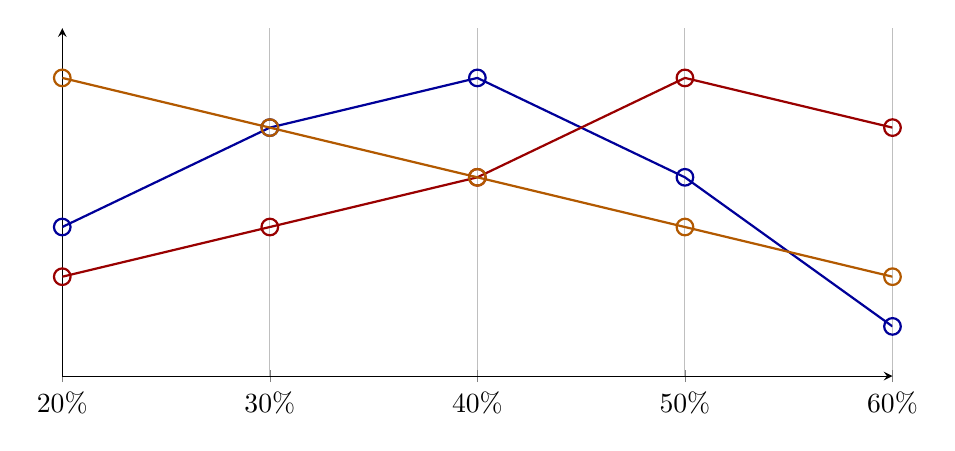
\begin{tikzpicture}
\begin{axis}[
    width=\linewidth,
    height=6cm,
    ymin=0,
    ymax=70,
    xmin=20,
    xmax=60,
    xtick={20,30,40,50,60},
    xticklabels={20\%,30\%,40\%,50\%,60\%},
    ytick=\empty,
    grid=major,
    axis lines=left,
    enlargelimits=false,
    legend style={draw=none},
]

% Alice
\addplot[
    color=blue!60!black,
    thick,
    mark=o,
    mark size=3pt,
    mark options={fill=white}
]
coordinates {
    (20,30)
    (30,50)
    (40,60)
    (50,40)
    (60,10)
};

% Bob
\addplot[
    color=red!60!black,
    thick,
    mark=o,
    mark size=3pt,
    mark options={fill=white}
]
coordinates {
    (20,20)
    (30,30)
    (40,40)
    (50,60)
    (60,50)
};

% Charlie
\addplot[
    color=orange!70!black,
    thick,
    mark=o,
    mark size=3pt,
    mark options={fill=white}
]
coordinates {
    (20,60)
    (30,50)
    (40,40)
    (50,30)
    (60,20)
};

\end{axis}
\end{tikzpicture}

\end{minipage}

\end{figure}

Here, as is a reasonable assumption,
the preferences of voters is 
single-peaked in some sense, 
according to the ordering of 
preference in the natural way.
Of course, there is not usually a natural way to order preferences.
We see more on single-peaked preferences later.
\end{example}

\begin{definition}
    A restricted domain $\mathcal{D}(U)$ is 
    a subset of $\mathcal{L}(U)^N$.
\end{definition}
\begin{example}
    \leavevmode \\
    \begin{itemize}
        \item The universal domain $\mathcal{D}_{\text{Univ}}(U) := \mathcal{L}(U)^N$.
        \item $\mathcal{D}_{\text{ab}}(U) = \set{R_N \in \mathcal{L}(U)^N : (\forall i \in N, a \succ_i b) \lor (\forall i \in N, b \succ_i a)}$
        is the domain where all voters agree on the relative ranking of $a$ and $b$.
    \end{itemize}
\end{example}

\begin{definition}
    A domain restriction $\mathcal{D}(U)$ is 
    \emph{Cartesian} if 
    $\mathcal{D}(U) = \mathcal{L}'(U)^N$ for some 
    $\mathcal{L}'(U) \subseteq \mathcal{L}(U)$.

    In a Cartesian domain, 
    the admissible preferences of a voter are independent of 
    the preferences of other voters (which need not be true).
\end{definition}

\section{Transitive Domains}

\begin{remark}
    $\mathcal{D}_\text{ab}(U)$ is not Cartesian,
    but $\mathcal{D}_\text{Univ}(U)$ is Cartesian.
\end{remark}

\begin{remark}
    As discussed, we use restricted domains to 
    bypass impossibility results. In particular, 
    we are interested in domain in which the majority
    relation $\gtrsim_M$ is transitive.

    It is clear that in this restricted domain, 
    $\succ_M$ contains no cycles, and so 
    we get rid of the Condorcet Paradox.

    In particular, 
    if $\gtrsim_M$ is transitive, then 
    $\operatorname{Max}(\gtrsim_M, A)$ is a well-defined SCF.
\end{remark}

\begin{comment}
    We often like to think of 
    (U, $\gtrsim_M$) as a graph.
\end{comment}


\begin{definition}
    Recall that an alternative $a \in U$ is 
    a Condorcet winner w.r.t preference profile 
    $R_N$ if $a \succ_M b$ for all $b \neq a$.

    We say that $a \in U$ is a weak Condorcet winner 
    w.r.t to $R_N$ if $a \gtrsim_M b$ for all $b \neq a$.
\end{definition}

\begin{proposition}
    If $\gtrsim_M$ is transitive, then 
    there exists a weak Condorcet winner.
\end{proposition}
\begin{proof}
    A transitive and complete relation on finite set has a maximum element.
\end{proof}

\begin{remark}
    We thus, motivate the domain 
    restricted to 
    just those profiles with transitive majority relation,
    since we have a natural SCF that just outputs
    the weak Condorcet winners.
    This, couldn't be done in the general case since 
    the Condorcet Paradox shows that we may have no 
    weak Condorcet winners.
\end{remark}

\begin{definition}
    Let $\mathcal{D}_{\text{TRANS}}(U) := \set{R_N \in \mathcal{L}(U)^N : \gtrsim_M \text{ is transitive}}$.

    As demonstrated if 
    $\gtrsim_M$ is transitive then
    $\operatorname{Max}(\gtrsim_M, A)$ is a well-defined SCF, 
    and its elements are exactly the weak Condorcet winners, 
    since they win or tie all pairwise majority comparisons.
\end{definition}

\begin{remark}
    $\mathcal{D}_{\text{TRANS}}(U)$ is not Cartesian.
\end{remark}

\begin{remark}
    In $\mathcal{D}_{\text{TRANS}}(U)$,
    the SCF $\operatorname{Max}(\gtrsim_M, A)$ 
    satisfies all the conditions of 
    Arrow's Theorem.
    
    It should be clear that 
    it is not a dictatoriship.

    Consider that if everyone ranks 
    one alternative over the other, 
    then 
    the majority must 
    strictly (in fact trivially) rank 
    that alternative over the other,
    and so clearly 
    $\operatorname{Max}(\gtrsim_M, A)$ satisfies Pareto optimality.

    Consider that if $A$
    is a feasible set and 
    $R_N, R_N'$ are two profiles that are the same when 
    restricted to $A$.
    Then consider that the pairwise majority
    in $R_N$ and $R_N'$ must be the same when restricted to $A$ (clearly).

    Finally, it is obvious that 
    the majority relation is a transitive 
    rationalisation of $\operatorname{Max}(\gtrsim_M, A)$.
\end{remark}

\begin{lemma}\label{l:majRelStratProofinTrans}
    $\operatorname{Max}(\gtrsim_M, A)$ is 
    strategyproof in $\mathcal{D}_{\text{TRANS}}(U)$.
\end{lemma}
\begin{proof}
    Suppose for contradiction 
    it is not.
    Then suppose that we have 
    two profiles 
    $R_N, R_N'$ that differ only in voter $i$'s preferences,
    and $A \in \mathcal{F}(U)$ such that
    $\operatorname{Max}(\gtrsim_M', A) \succ_i \operatorname{Max}(\gtrsim_M, A)$
    where $\operatorname{Max}(\gtrsim_M', A), \operatorname{Max}(\gtrsim_M, A)$ are singletons.
    That is there is only one weak condorcet winner.

    Let $a$ be the weak Condorcet winner in $R_N$ and $a'$ be the weak Condorcet winner in $R_N'$.
    Thus, $a \succ_M a'$, $a' \succ_M' a$ (strictly because 
    otherwise $a'$ (resp. $a$) would also be weak 
    condorcet winners, contradicting uniqueness), and $a' \succ_i a$.
    But then, consider that since $a \succ_M a'$, and $a' \succ_i a$, and 
    $R_N$ and $R_N'$ differ only in voter $i$'s preferences, the relative 
    ranking in $i$'s preferences between 
    $a$ and $a'$ can only keep the same relative ranking or promote 
    $a$ compared to $a'$. Thus, it must be that 
    $a \succ_M' a'$. Contradiction.

\end{proof}

\begin{corollary}
    If $\mathcal{D}(U)$ is a subdomain of 
    $\mathcal{D}_{\text{TRANS}}(U)$ (i.e.
    $\mathcal{D}(U) \subseteq \mathcal{D}_{\text{TRANS}}(U)$)
    then clearly the same proof above follows, 
    and so we get that 
    $\operatorname{Max}(\gtrsim_M, A)$ is strategyproof in $\mathcal{D}(U)$.
\end{corollary}


\begin{remark}
    If there are an odd number of voters, 
    then $\operatorname{Max}(\gtrsim_M, A)$ is resolute in $\mathcal{D}_{\text{TRANS}}(U)$.
\end{remark}
\begin{proof}
    Clear. Cannot be that $n_{ab} = n_{ba}$.
\end{proof}

\begin{theorem}[Cambell and Kelly, 2003]
    If $n$ is odd, $\operatorname{Max}(\gtrsim_M, A)$ is the only SCF that is
    non-dictatorial, Pareto-optimal, strategyproof, and
    resolute in $\mathcal{D}_{\text{TRANS}}(U)$.
\end{theorem}
\begin{proof}
    Omitted.
\end{proof}


\section{Single-Peaked Domains}


We see that the domain 
$\mathcal{D}_{\text{TRANS}}(U)$ is a nice domain to work with,
but perhaps it feels like a contrived example, 
we now turn to a natural example of a domain that is 
a subdomain of $\mathcal{D}_{\text{TRANS}}(U)$.

\begin{definition}
    Let $\trianglelefteq \ \in \mathcal{L}(U)$ be a linear order of alternative.
    A preference relation $\gtrsim \in \mathcal{L}(U)$ is \emph{single-peaked with respect to $\trianglelefteq$}
    if
    for all $x, y, z \in U$:
    ((x $\triangleleft$ y $\triangleleft$ z) or (z $\triangleleft$ y $\triangleleft$ x)) implies
    ($x \succ y \implies y \succ z$).

    This says, that if the linear order 
    ranks 
    $y$ between $x$ and $z$, 
    then if the preference relation ranks $x$ over $y$, then it must rank $y$ over $z$.
    This gives a kind of monotonicity condition everywhere 
    except for when 
    the linear order ranks $y$ at the top of $x$ and $z$, in which case there is no restriction, 
    and $y$ may be the peak.

    Alternatively, consider what this definition forbids.
    That is, it disallows the middle 
    alternative from being ranked lowest (think this over).
\end{definition}

\begin{definition}
    For a linear order $\trianglelefteq \ \in \mathcal{L}(U)$,
    and a preference profile 
    $R_N \in \mathcal{L}(U)^N$,
    we say that 
    $R_N$ is \emph{single-peaked with respect to $\trianglelefteq$}
    if each preference relation in $R_N$ is single-peaked with respect to $\trianglelefteq$.
\end{definition}


\begin{definition}
    We define the 
    \emph{domain of single-peaked preferences}
    with respect to $\trianglelefteq$ as
    \[    \mathcal{D}_{\text{SP}}^{\trianglelefteq}(U) := \set{R_N \in \mathcal{L}(U)^N : R_N \text{ is single-peaked with respect to } \trianglelefteq} \]

    
    Equivalently, 
    we can define 
    it as
    \[
        \mathcal{D}_{\text{SP}}^{\trianglelefteq}(U) := \set{\gtrsim \in \mathcal{L}(U) : \gtrsim \text{ is single-peaked with respect to } \trianglelefteq}^N
    \]
    Clearly, under this definition we see that 
    $\mathcal{D}_{\text{SP}}^{\trianglelefteq}(U)$ is Cartesian.
\end{definition}

\begin{remark}
    Single-peaked arises naturally in a few situations,
    \begin{itemize}
        \item The desired distance of a train station from 
        your house
        \item Left-Right political spectrum
        \item Age for people to be allowed to vote
    \end{itemize}
\end{remark}

The big motivation for 
considering single-peaked preferences, is the following 
theorem, which follows from the previous section.
\begin{theorem}[Black, 1948]
    $\gtrsim_M$ is transitive in 
    $\mathcal{D}_{\text{SP}}^{\trianglelefteq}(U)$.

    \begin{itemize}
        \item In particular, if $n$ is odd, every single-peaked profile 
        admits a (strict) Condorcet winner.
        \item For even $n$, weak Condorcet winners are guaranteed
    \end{itemize}
\end{theorem}

We defer the proof to ???, from which it follows trivially.


\begin{remark}
    The above also holds for so-called, 
    \emph{single-caved} preferences $\mathcal{D}_{\text{SC}}^{\trianglelefteq}(U)$.
    A preference relation $\gtrsim$ is single-caved with respect to $\trianglelefteq$ if for all $x, y, z \in U$:
    ((x $\triangleleft$ y $\triangleleft$ z) or (z $\triangleleft$ y $\triangleleft$ x)) implies
    ($y \succ x \implies z \succ y$).   
\end{remark}

\begin{theorem}
    We give some intuition as to why
    $\gtrsim_M$ is transitive in $\mathcal{D}_{\text{SP}}^{\trianglelefteq}(U)$.

    Assume that $n$ is odd, 
    let $t_i$ denote the alternative ranked highest
    by voter $i$ (the \emph{top-choice} of voter $i$).
    We can imagine placing pebbles 
    along the linear order $\trianglelefteq$ for each voter 
    according to their top choice.
    Then the alternative that the
    median pebble (according to $\trianglelefteq$) is placed on is the Condorcet winner.
\end{theorem}
\begin{proof}
    \unclear{TODO: Easy proof.}
\end{proof}

\begin{remark}
    This proves something that is just a 
    slightly weaker Black's theorem.
\end{remark}

\begin{remark}[Median Voting]
    By the above,
    that just the voters'
    top choices are sufficient 
    to compute the Condorcet winner (when one exists).
    
    \begin{quote}
        Importantly, we note that 
        the plurality winner may differ from the 
        Condorcet winner, 
        even in $\mathcal{D}_{\text{SP}}^{\trianglelefteq}(U)$.
    \end{quote}
    
    In the domain $\mathcal{D}_{\text{SP}}^{\trianglelefteq}(U)$
    this --- which is just
    $\operatorname{Max}(\gtrsim_M, A)$ --- 
    is known as \emph{median voting}.

    Median voting satisfies 
    strategyproofness in the domain $\mathcal{D}_{\text{SP}}^{\trianglelefteq}(U)$.
    This follows from Black's theorem and Lemma~\ref{l:majRelStratProofinTrans}.

    In $\mathcal{D}_{\text{SP}}^{\trianglelefteq}(U)$,
    it is computationally trivial to find the Condorcet winner.
    So far, we have not thought much about the 
    computational social choice theory from a complexity perspective,
    but this is a theme of the course that we will now be seeing more of.
\end{remark}

\begin{remark}
    \textsc{Can we efficiently check whether a preference profile is 
    single-peaked with respect?}
    If we are given some order 
    $\trianglelefteq$, we can trivially check whether a preference profile is single-peaked with respect to $\trianglelefteq$
    by verifying the single-peaked condition for each voter's preferences 
    We check the single-peaked condition for each preference relation in a profile 
    by going through each voter's contiguous 3-tuples of preferences (think!) i.e. in time linear in 
    the number of alternatives.
    Thus, given $\trianglelefteq$, we can check whether a profile is single-peaked with respect to $\trianglelefteq$
    in time $O(n|U|)$.

    The more interesting question is 
    whether we can efficiently check single-peakedness without being given $\trianglelefteq$;
    after all, we have all these nice properties 
    if a profile is single-peaked with respect to some order,
    so it is nice to be able to easily check whether a profile is single-peaked.
    Of course, checking all linear orders is not efficient.
\end{remark}

\begin{observation}
    A least-ranked alternative in a preference relation
    must be placed at the leftmost or rightmost end of the linear order.
    \unclear{Reason why this is true?}
    Thus, there can be at most two least-ranked alternatives.
    This motivates the idea that we try to arrange the alternatives from the outside to the inside.
\end{observation}

\begin{idea}
    From this, we attempt to construct a linear order 
    by placing the least-ranked alternatives at the ends, 
    and iterating this.
    Suppose that after one iteration 
    $l$ and $r$ are the least-ranked alternatives in the profile and 
    so they get placed at the innermost left and right positions of 
    the partially constructed linear order.
    Then, we remove $l$ and $r$ from the profile and repeat this process.
    Let $A \subseteq U$ be the set of alternatives that have not yet been arranged.

    Suppose that $x$ is the bottom ranked alternative in
    the profile restricted to $A$ (so needs to be placed next).
    If there is a voter that ranks
    $l \succ_i x \succ_i r$, and 
    that voter does not rank $x$ as their top choice when 
    we restrict to $A$, then we have to place 
    $x$ on the right (next to $r$).

    Why?

    
    Suppose for contradiction that $x$ is placed on the left, 
    just inside $l$. Then in $\trianglelefteq$ the arrangement is:
    \[
        \cdots \quad l \quad x \quad \underbrace{A \setminus \set{x}}_{\ni\; t_i} \quad r \quad \cdots
    \]
    where $t_i$ denotes the peak of voter $i$ restricted to $A$,
    which is not $x$ by assumption.
    Since $t_i \in A \setminus \{x\}$, 
    it lies strictly to the right of $x$ in $\trianglelefteq$.
    Moving leftward from $t_i$, 
    we reach $x$ before $l$, 
    so $x$ is closer to $t_i$ than $l$ is.
    Single-peakedness then requires $x \succ_i l$.
    But voter $i$ has $l \succ_i x$, a contradiction.
    Thus $x$ must be placed on the right, next to $r$.
    \unclear{Check this makes sense.}
\end{idea}

\begin{algorithm}[H]
\caption{Single-Peaked Recognition}
\begin{algorithmic}[1]
\State Set dummy leftmost alternative to $z_l \notin U$, rightmost to $z_r \notin U$
\State $l \gets z_l$, $r \gets z_r$
\State $A \gets U$
\While{$|A| \geq 2$}
    \State $B \gets \{x \in A : x \text{ is bottom-ranked in } R_N|_A \text{ for some voter}\}$
    \State $R \gets \{x \in B : \exists i \in N \text{ such that } l \succ_i x \succ_i r \text{ and } t_i(A) \neq x\}$
    \State $L \gets \{x \in B : \exists i \in N \text{ such that } r \succ_i x \succ_i l \text{ and } t_i(A) \neq x\}$
    \If{$|B| \leq 2 \land |L| \leq 1 \land |R| \leq 1 \land L \cap R = \emptyset$}
        \State Place the alternative in $L$ (if any) next to $l$; update $l$
        \State Place the alternative in $R$ (if any) next to $r$; update $r$
        \State Place any $x \in B \setminus (L \cup R)$ in an arbitrary empty slot next to $l$ or $r$
    \Else
        \State \Return $R_N$ is not single-peaked
    \EndIf
    \State $A \gets A \setminus B$
\EndWhile
\If{$|A| = 1$}
    \State Place the remaining $x \in A$ in the last slot
\EndIf
\State \Return $R_N$ is single-peaked with the constructed order $\trianglelefteq$
\end{algorithmic}
\end{algorithm}
\unclear{TODO: Write and understand this in more detail, also trace this algorithm for an example.}

\begin{theorem}
    The above algorithm 
    is correct and 
    runs in time $O(n|U|)$ 
    --- so in time that is linear in 
    in the size of a specification of 
    a preference profile.
\end{theorem}
\begin{proof}
    See~\cite{ElkindLP2022}[Section 4.1.].
\end{proof}

\begin{remark}
    Essentially the same algorithm
    can be used to check whether a profile is single-caved,
    by running it on a preference profile that is flipped upside down.
\end{remark}

\begin{remark}
    We have noted that
    $\gtrsim_M$ is 
    transitive in 
    $\mathcal{D}_{\text{SP}}^{\trianglelefteq}(U)$
    and in 
    $\mathcal{D}_{\text{SC}}^{\trianglelefteq}(U)$.
    Therefore, it is too in the 
    union domain, 
    \[
        \mathcal{D}_{\text{SP}}^{\trianglelefteq}(U) \cup \mathcal{D}_{\text{SC}}^{\trianglelefteq}(U)
    \]

    One might ask if this is maximal, 
    that is, do there exist
    profiles that are neither 
    single-peaked nor single-caved,
    which still have a transitive 
    majority relation?
    The answer is no, 
    consider the following example.

    \begin{center}
    \begin{tabular}{|c|c|c|}
        \hline
        \textbf{1} & \textbf{1} & \textbf{1} \\
        \hline
        $b$ & $a$ & $d$ \\
        $c$ & $b$ & $b$ \\
        $a$ & $c$ & $c$ \\
        $d$ & $d$ & $a$ \\
        \hline
    \end{tabular}
    \end{center}

    That is because, the above profile 
    satisfies the 
    property of 
    \emph{single-peakedness for triples} --- defined in a rather obvious way.

    Can we characterise the (Cartesian) domains for which the 
    majority relation is transitive \footnote{
        We restrict to Cartesian domains, otherwise by definition it is 
        just $\mathcal{D}_{\text{TRANS}}$.
    }?

\end{remark}

\begin{definition}[Value-Restricted Domain]
    A Cartesian domain $\mathcal{D}(U) = \mathcal{L}'(U)^N$ with 
    $\mathcal{L}'(U) \subseteq \mathcal{L}(U)$ is 
    \emph{value-restricted} if for each $x, y, z \in U$, 
    there is some alternative, say $x$, such that
    \begin{itemize}
        \item $x$ is never the worst alternative 
        ($\forall \gtrsim \in \mathcal{L}'(U): x \succ y \lor x \succ z$), or
        \item $x$ is never the best alternative 
        ($\forall \gtrsim \in \mathcal{L}'(U): y \succ x \lor z \succ x$), or
        \item $x$ is never the middle alternative 
        ($\forall \gtrsim \in \mathcal{L}'(U): (x \succ y \land x \succ z) \lor (y \succ x \land z \succ x)$).
    \end{itemize}

    The forbidden substructure for value-restricted domains is 
    the Condorcet profile restricted to any triple:
    \begin{center}
    \begin{tabular}{ccc}
        $x$ & $y$ & $z$ \\
        $y$ & $z$ & $x$ \\
        $z$ & $x$ & $y$
    \end{tabular}
    \end{center}

    $\mathcal{D}_{\text{SP}}^{\trianglelefteq}(U)$ and 
    $\mathcal{D}_{\text{SC}}^{\trianglelefteq}(U)$ are value-restricted 
    for all $\trianglelefteq$.
\end{definition}

\begin{theorem}[Sen and Pattanaik, 1969]
    Let $\mathcal{L}'(U) \subseteq \mathcal{L}(U)$ and $n$ odd.
    Then, $\gtrsim_M$ is transitive in domain 
    $\mathcal{D}(U) = \mathcal{L}'(U)^N$ iff $\mathcal{D}(U)$ is value-restricted.
\end{theorem}

\begin{remark}
    This does \textbf{not} imply that every preference profile 
    for which $\gtrsim_M$ is transitive, is value-restricted.
    For example, consider the following profile:
    \begin{center}
    \begin{tabular}{|c|c|c|}
        \hline
        \textbf{3} & \textbf{1} & \textbf{1} \\
        \hline
        $a$ & $b$ & $c$ \\
        $b$ & $c$ & $a$ \\
        $c$ & $a$ & $b$ \\
        \hline
    \end{tabular}
    \end{center}
    Here $\gtrsim_M$ is transitive (since $a$ wins every pairwise comparison),
    yet $\mathcal{L}'(U) = \mathcal{L}(U)$ contains the full Condorcet triple,
    so the domain is not value-restricted.
\end{remark}

\chapter{Borda, Condorcet, and Kemeny}

\begin{idea}    
    The \emph{theme} of this chapter
    comes from the conflict between 
    the social choice ideas of 
    Borda and Condorcet.
\end{idea}

\begin{definition}
    In this chapter,
    we consider a variable set of voters.

    Formally speaking, 
    we consider the set of preference profiles over 
    $\bigcup_{N \subseteq \mathbb{N}; |N| < \infty} \mathcal{L}(U)^N$.
    This allows us to 
    consider profiles with different numbers of voters, and 
    consider merging
    profiles $R_N \in \mathcal{L}(U)^N$
    and $R_{N'} \in \mathcal{L}(U)^{N'}$ into a profile $R_{N} \cup R_{N'} \in \mathcal{L}(U)^{N \cup N'}$
    (assuming $N \cap N' = \emptyset$).
\end{definition}

\begin{definition}[Scoring Rule]
    Informally speaking, 
    for a fixed feasible set 
    $A \subseteq U$,
    a \emph{score vector} $s := (s_1, s_2, \ldots, s_{|A|})$ is a real vector, 
    such that if voter ranks an alternative 
    at the $i$-th position, then it gets $s_i$ points.
    A \emph{scoring rule} is a SCF that choses those 
    alternatives with the highest total score.

    More formally, 
    we should define the notion of a score vector for each possible size of feasible set.
    Let 
    $s^{(1)}, s^{(2)}, \ldots, s^{(|U|)}$
    be a collection of score vectors where 
    $s^{(k)}$ has size $k$.
    The corresponding scoring rule is defined as
    $\operatorname{argmax}_{x \in A} s(x, A)$, 
    where, 
    \[
        s(x, A) := \sum_{i \in N} s_{|y \in A: y \gtrsim_i x|}^{(|A|)}
    \]

\end{definition}

\begin{remark}
    The above definition is a bit weird/annoying, 
    it allows for perversities like 
    Borda for even sized 
    feasible sets and Plurality for odd sized feasible sets.
    Usually, we think about the feasible set as fixed and 
    often omit it from the notation.
\end{remark}

\begin{example}
    \leavevmode \\
    \begin{itemize}
        \item 
        Borda's rule, 
        $s^{(|A|)} := (|A| - 1, |A| - 2, \ldots, 0)$.
        \unclear{Think if this is broad or narrow Borda?}

        \item Plurality, $s^{(|A|)} := (1, 0, \dots, 0)$
        
        \item \emph{Anti-Plurality}, 
        $s^{(|A|)} := (1, 1, \ldots, 1, 0)$
    \end{itemize}
\end{example}

\begin{proposition}\label{p:scoring-rules-affine}
    Scoring rules are 
    invariant under \emph{positive affine transformations}
    \footnote{$s_i^{(k)} \mapsto \alpha_i s_i^{(k)} + \beta_i$ where $\alpha_i > 0$.}
    of their score vectors.
\end{proposition}
\begin{proof}
    Easy boring exercise.
\end{proof}

\begin{proposition}
    Scoring rules can be efficiently computed \footnote{Meaning it is in $\mathbf{P}$.}.
\end{proposition}
\begin{proof}
    We compute them in the obvious way.
\end{proof}

\begin{proposition}
    A scoring rule is monotonic 
    if and only if 
    for all $k$, $s_1^{(k)} \geq s_2^{(k)} \geq \ldots \geq s_k^{(k)}$.

    A monotonic 
    scoring rule is \emph{non-trivial}
    if $s_1^{(k)} > s_k^{(k)}$.
\end{proposition}
\begin{proof}
    Exercise.
\end{proof}

\begin{definition}[Reinforcement]
    A SCF $f$ satisfies \emph{reinforcement}
    if for all $A$ and 
    disjoint sets 
    of voters $N$ and $N'$,
    and all 
    $R_N \in \mathcal{L}(U)^N$ and $R_{N'} \in \mathcal{L}(U)^{N'}$,
    such that 
    $f(R_N) \cap f(R_{N'}) \neq \emptyset$, 
    \[
        f(R_N \cup R_{N'}, A) = f(R_N, A) \cap f(R_{N'}, A)
    \]
    Informally, 
    whenever there is a common alternative selected by two disjoint sets 
    of voters (under the SCF), 
    then the common alternatives should be the only
    alternatives selected when we merge the two sets of voters together.
\end{definition}


\begin{example}
    Let's think about which rules satisfy this.
    It is clear that Plurality satisfies this.
    \unclear{Think why? Also, does Borda satsify it?}
\end{example}

\begin{theorem}[Smith, 1973; Young, 1975]
    A neutral and 
    anonymous 
    SCF satisfies 
    reinforcement if and only if it is a \emph{composed} scoring rule.
\end{theorem}

\begin{definition}[Composed scoring rule]
    An SCF is a \emph{composed} scoring rule if there is 
    (finite) sequence 
    of scoring rules 
    where each scoring rules (if there is a next scoring rule) 
    is used to 
    break ties, 
    (if there are any), 
    of the previous rule.

    Any scoring rule is a 
    composed scoring rule,
    by taking the length of the sequence to be one.
\end{definition}

\begin{intuition}
    Roughly speaking, 
    reinforcement characterises 
    scoring rules (composed) --- sometimes 
    reinforcement can be used to reason about 
    all scoring rules.
\end{intuition}

\begin{definition}[Cancellation]
    An SCF satisfies \emph{cancellation} if for all $A$ and
    $R_N$, 
    \[
        \bigg( 
            \forall x, y \in A: n_{xy} = n_{yx}
        \bigg)
        \implies
        f(R_N, A) = A
    \]
    NB: Cancellation is only meaningful when $n$ is even.
\end{definition}

\begin{remark}
    Borda is a scoring rule which satisfies cancellation.
    To see as such, 
    consider we can alternatively formulate
    the total Borda score $s_{\text{NarrowBorda}}(x, A)$ 
    of alternative $x$ as, 
    the sum of the number of voters that 
    rank $y \neq x$ below $x$ for each alternative $y$, i.e., 
    \[
        s_{\text{NarrowBorda}}(x, A) = \sum_{y \in A \setminus \{x\}} n_{xy}
    \]
    This is just changing the order of summation from 
    summing first over alternatives and then over 
    voters to the reverse order.
    As such, we see that if 
    for all $x, y \in A$, $n_{xy} = n_{yx}$, then
    clearly 
    $s_{\text{NarrowBorda}}(x, A) = s_{\text{NarrowBorda}}(y, A)$ for all $x, y \in A$,
    and so 
    $f(R_N, A) = A$.
\end{remark}

\begin{remark}
    Plurality does not satisfy cancellation.
    Consider the profile on three alternatives with two voters where one voter
    has preferences 
    $a \succ_1 b \succ_1 c$
    and the other has 
    the reverse $c \succ_2 b \succ_2 a$.
    Then, for the total feasible set
    $A = \{a, b, c\}$,
    $n_{ab} = n_{ba} = 1$,
    $n_{ac} = n_{ca} = 1$, and
    $n_{bc} = n_{cb} = 1$,
    so the cancellation condition is satisfied, but
    $f(R_N, A) = \{a, c\} \neq A$.
\end{remark}

\begin{theorem}[Young, 1974]
    Borda's (narrow) rule 
    is the only SCF satisfying 
    neutrality, Pareto-optimality, 
    reinforcement, 
    and cancellation.
\end{theorem}

\section{Family of Condorcet Extensions}

\begin{definition}
    An SCF $f$ is a \emph{Condorcet extension} 
    if it picks a the (strict) Condorcet winner 
    whenever there is one, and otherwise does something (anything) else.
\end{definition}

\unclear{Can you think of a SCF which is a Condorcet extension?}

\subsection{Fishburn's Classification}

\begin{idea}
    Fishburn's Classification is used to
    categorise Condorcet Extensions based on the 
    amount of \emph{information} used to compute them.
\end{idea}

\begin{definition}[C1 Graph]
    The \emph{C1 Graph} or \emph{Majority Graph}
    with respect to a preference profile 
    $R_N$ is the directed graph with vertex set $U$ and
    and edge from 
    $a$ to $b$ if $a \succ_M b$.
    That is, the edges are given by the majority relation,
    where there is an edge from $a$ to $b$ iff 
    $a$ strictly wins the pairwise majority comparison with
    $b$.
\end{definition}

\begin{definition}[C2 Graph]
    The \emph{C2 Graph} or \emph{Weighted Majority Graph}
    is the directed graph with vertex set $U$ and
    edges from $a$ to $b$ with weight $n_{ab}$.
\end{definition}

\begin{remark}
    It is clear that 
    we can extract the 
    C1 Graph from the 
    C2 Graph by just looking at the edge weights
    and seeing whether an edges has weight greater than the reverse edge.
\end{remark}

\begin{definition}[Margin Graph]
    The \emph{Margin Graph} is the directed graph with vertex set $U$
    and an edge from 
    $a$ to $b$ with weight $n_{ab} - n_{ba}$
    whenever $n_{ab} > n_{ba}$.
\end{definition}

\begin{remark}
    It is clear that
    the margin graph has precisely the same edges as
    the C1 graph, but with weights given by the margin of victory.
\end{remark}

\begin{definition}[Fishburn's Classification]
    Fishburn classifies 
    Condorcet extensions 
    (and more generally SCFs)
    into three classes
    C1, C2, and C3.
    \begin{itemize}
        \item \textbf{C1:} $f$ depends only on the
        majority relation, that is it is a function of 
        the C1 Graph.
        \item \textbf{C2:} $f$ depends only on the
        weighted majority relation
        and is not in C1, that is it is a function of
        the C2 Graph (but not just the C1 Graph).
        \item \textbf{C3:} $f$ is 
        not a function of the C2 Graph (and hence it is not C1 nor C2).
    \end{itemize}
\end{definition}

\begin{example}[Copeland's Rule]
    We define Copeland's Rule as, 
    \[
        f_{\text{Copeland}}(R_N, A) := \operatorname{argmax}_{x \in A} |\{y \in A 
        : x \succ_M y\}|
    \]
    That is, the Copeland rule gives those alternatives that win 
    the most pairwise majority comparisons.
    
    The Copeland rule is a C1 rule, since it depends only on the majority relation.
    We can see that the Copeland rule can be thought of as returning all those 
    alternatives that have the maximal outgoing edges in the C1 graph.

    We also note, that the Copeland Rule is a Condorcet extension, 
    since if there a Condorcet winner, 
    i.e. an alternative that wins all pairwise majority comparisons, 
    then it is the unique alternative with the most outgoing edges in the C1 graph, and so it is the unique winner under the Copeland Rule.
\end{example}

\begin{example}[Maximin Rule]
    We define the Maximin rule as, 
    \[
        f_{\text{Maximin}}(R_N, A) := \operatorname{argmax}_{x \in A} \min_{y \in A \setminus \{x\}} n_{xy}
    \]
    That is, the Maximin rule gives those alternatives whose weakest pairwise majority victory is as strong as possible.

    The Maximin rule is a C2 rule, since it depends on the weighted majority relation, but not just the majority relation.
    We can see that the Maximin rule can be thought of as returning all those alternatives that have the maximal weight
    on their weakest outgoing edge in the C2 graph.

    Let us pause to think how we would formally show that it is a C2 rule.
    We would exhibit profiles that have identical 
    C1 Graphs, but for which the maximin rule differs.

    We also note, that the Maximin Rule is a Condorcet extension, 
    since it must win in the majority relation, so 
    if there is a Condorcet winner $a$, it must be that 
    $n_{ay} > n_{ya}$ for all $y \neq a$, so 
    $n_{ay} > n/2$.
    For any other alternative $x \neq a$, 
    then since $n_{ax} > n/2$
    and there are $n$ voters, it must be that $n_{xa} < n/2$.
\end{example}

\begin{example}[Borda's (narrow) Rule]
    We note that, 
    Borda's (narrow) rule is given by, 
    \[
        f_{\text{Borda}}(R_N, A) := \operatorname{argmax}_{x \in A} \sum_{y \in A \setminus \{x\}} n_{xy}
    \] 
    Thus clearly it is a C2 rule, since it depends on the weighted majority relation.
    On the C2 graph, we compute the Borda winners as those 
    alternatives that have the maximal total outgoing edge weight.

    It should be noted that Borda's
    rule is \textbf{not} a Condorcet extension.
    \unclear{Think why?}
\end{example}

\begin{example}
    Plurality is a C3 rule, since it is not a function of the C2 graph.
    \unclear{Come up with two profiles with identical 
    C2 Graphs but differing Plurality winners}
    \unclear{Aside from Borda's rule what other (if any) scoring rules are in C1, C2, and C3}.
\end{example}

\begin{example}[Young's Rule]
    Returns all alternatives that can be made a (strict) Condorcet Winner
    when we remove a minimal number of voters.
    That is, over each alternative, what is the fewest number of 
    voters we need to remove to make that alternative a Condorcet winner,
    and then we return those alternatives for which this number is minimal.

    Young's rule is obviously a Condorcet extension.
    Young's rule is intractible.
    Young's rule is a C3 rule, for some intuition for why it is not 
    C2, to know what voters to delete, we need to have access to the 
    rankings in the profile (try to prove it formally).
\end{example}

\begin{remark}
    When there are only two alternatives, majority rule
    (which is just plurality) is the 
    the only non-trivial, monotonic scoring rule, 
    and the only Condorcet extension.
\end{remark}

\begin{proposition}[Condorcet, 1785]
    Borda's rule is not a Condorcet extension
    when there are three or more alternatives.
\end{proposition}
\begin{proof}
    First for the case of three alternatives consider the profile
    given by 
    four voters having preferences 
    $a \succ b \succ c$,
    and three voters having 
    $b \succ c \succ a$.
    Then $a$ gets a total Borda score of $4 \cdot 2 + 3 \cdot 0 = 8$,
    and $b$ gets a total Borda score of $4 \cdot 1 + 3 \cdot 2 = 10$.
    So Borda's rule does not select $a$. 
    Despite this, $a$ is the Condorcet winner, since $a$ beats $b$  and $c$ by 4 votes to 3.

    Now in general suppose there are 
    $m \geq 3$ alternatives and consider the profile given by 
    $n_1$ voters having 
    preference relations $P_1: a \succ b \succ \cdots$,
    and $n_2$ voters having
    preference relations $P_2: b \succ  \cdots \succ a$.
    For $a$ to be a Condorcet winner, we need $n_1 > n_2$.
    Consider that 
    $a$ gets a total Borda score of 
    $n_1 \cdot (m - 1) + n_2 \cdot 0 = n_1(m - 1)$,
    and $b$ gets a total Borda score of
    $n_1 \cdot (m - 2) + n_2 \cdot (m - 1)$.
    We can thus ensure that $b$ has a higher 
    Borda score than $a$ and that 
    $a$ is the Condorcet winner by choosing $n_1$ and $n_2$ such that
    $n_2 < n_1 < (m-1)n_2$, 
    for $m \geq 3$ this can be achieved easily.

    Hence, we can construct a profile where $a$ is the Condorcet winner but $b$ has a higher Borda score,
    and so Borda's rule does not select the Condorcet winner for 
    each $m \geq 3$ (observe the inequality fails when $m = 2$).
    The above example for $m = 3$ does exactly this.
\end{proof}

\begin{theorem}
    No scoring rule is a Condorcet extension when 
    there are three or more alternatives.
\end{theorem}
\begin{proof}
    Exercise.
    (Hint: Condition first on monotonic and non-monotonic scoring rules,
    maybe use Proposition~\ref{p:scoring-rules-affine}
    and then construct profiles.)
\end{proof}

\begin{remark}
    We could think of Borda scoring as giving points per rank, 
    and describe Borda's rule as choosing the alternatives with the highest average rank.
\end{remark}

\begin{theorem}[Smith, 1973]
    A Condorcet winner is 
    never the alternative with the lowest Borda score.
    Borda's rule is the 
    only scoring rule for which this 
    holds.
    
    We can think of this as saying that 
    Borda is the scoring rule which is most compatible with 
    the Condorcet criterion.


    Equivalently, a Condorcet loser 
    \footnote{An alternative $x$ is a Condorcet loser if it strictly loses all non-reflexive pairwise majority comparisons.}
    is never the alternative with the 
    highest Borda score (and again the only scoring rule for which this works is Borda's).
\end{theorem}
\begin{proof}
    Exercise.
\end{proof}

\begin{theorem}[Gehrlein et al., 1978]
    When all preferences profiles are equally likely, 
    over all scoring rules, Borda's rule maximizes
    the probability of selecting the Condorcet winner (when one exists).
\end{theorem}

\begin{idea}[Unifying Borda and Condorcet]
    Despite there being conflict between 
    Borda and Condorcet there have been some attempts to unify the rules.
    \begin{itemize}
        \item Black's Rule: Return the Condorcet winner when 
        one exist, otherwise the Borda winner(s) (by definition a Codorcet extension).
        - it is slightly ad hoc.
        \item Baldwin's Rule:
        Run-off method based on (narrow) Borda's rule.
        In each round, all the minimal (narrow) Borda score alternatives are deleted, 
        until no more deletions are possible --- output this set now.
        Baldwin's rule is a Condorcet extension (Exercise), 
        but it is not monotonic
        \footnote{Every scoring run-off rule violates monotonicity (Smith, 1973)}.
    \end{itemize}
\end{idea}

\begin{theorem}[Young and Levenglick, 1978]\label{t:Young-Levenglick}
    For three or more alternative, no Condorcet extension satisfies reinforcement
    
\end{theorem}
\begin{proof}
    Assume for contradiction that $f$ is an SCF which is 
    a Condorcet extension satisfying 
    reinforcement.
    Consider the profile $R_N$ given below,
    \begin{center}
    \begin{tabular}{c|c|c}
        $a \succ b \succ c$ & $b \succ c \succ a$ & $c \succ a \succ b$ \\
        2 voters & 2 voters & 2 voters
    \end{tabular}
    \end{center}
    Since $f(R_N, \set{a, b, c})$ must select 
    some alternative and the profile is symettric in 
    $a$, $b$, and $c$, there is no Condorcet winner, 
    so without loss of generality assume 
    $b \in f(R_N, \set{a, b, c})$.

    Consider the profile $R_{N'}$ below,
    \begin{center}
    \begin{tabular}{c|c}
        $b \succ a \succ c$ & $a \succ b \succ c$ \\
        2 voters & 1 voter
    \end{tabular}
    \end{center}

    Then, in $R_{N'}$, $b$ is 
    the Condorcet winner, so $f(R_{N'}, \set{a, b, c}) = \{b\}$.
    By reinforcement, $f(R_N \cup R_{N'}, \set{a, b, c}) = f(R_N, \set{a, b, c}) \cap f(R_{N'}, \set{a, b, c}) = \{b\}$.
    
    Now, consider the combined profile, 
    here $a$ is the Condorcet winner, so 
    $f(R_N \cup R_{N'}, \set{a, b, c}) = \{a\}$.
    Contradiction.

    It is convenient in this proof to draw the 
    margin graphs for 
    $R_N$ and $R_{N'}$, then we can easily 
    combine them to get the 
    margin graph for $R_N \cup R_{N'}$.
\end{proof}

\begin{idea}
    To prove this for a general number of alternatives,
    we can \emph{cheat} by adding extra preferences at the bottom
    of the profiles $R_N$ and $R_{N'}$, and taking the same feasible set.
    Exercise: can we show that the theorem holds for the total 
    feasible set on any number of alternatives greater than three.

    Usually, when something goes wrong for some number of alternatives, 
    it does for larger numbers of alternatives too --- so it is interesting when it first goes wrong, 
    which is usually for three alternatives (majority is axiomatically nice for two alternatives).
\end{idea}

\begin{idea}[Social Preferences]
    SPF : $\mathcal{L}(U)^N \to \mathcal{F}(\mathcal{L}(U))$, 
    where $\mathcal{F}(\mathcal{L}(U))$ is the set of non-empty finite subsets of $\mathcal{L}(U)$.

    In this context, 
    Young and Levenglick's theorem (Theorem~\ref{t:Young-Levenglick})
    doesn't hold.
\end{idea}

\section{Kemeny's Rule}


\begin{definition}[Social Preference Functions]
    A \emph{social preference function} (SPF) is a function $h$
    that maps a preference profile to a non-empty set of linear orders over $U$.
    That is, 
    \[
        h : \mathcal{L}(U)^N \to \mathcal{F}(\mathcal{L}(U))
    \]
    We can think of a 
    social preference function as a generalisation of a social welfare function,
    where we can output a set of orders instead of just one, 
    and where the orders must be linear orders instead of just weak orders.
\end{definition}

\begin{definition}[Kemeny's Rule]
    Kemeny's rule is 
    a SPF defined as,
    \[
        h_{\text{Kemeny}}(R_N) := \operatorname{argmax}_{\gtrsim \in \mathcal{L}(U)} \sum_{i \in N} |\{\langle x, y\rangle : x \succ y, x \succ_i y\}|
    \]
    As with SCFs, we approach them from 
    an optimization perspective.
    Here, instead of optimizing over 
    alternatives, we optimize over linear orders.

    Informally, for each linear order, 
    we give it points based on how much it agrees with 
    a voters preference, and sum over all voters, and then we return (all) those linear orders that have the highest total score.

    NB: We can think about Kemeny's rule as that which yields all rankings that 
    maximize agreement with the profile. More intuitively, we can think about it minimizing the 
    pairwise disagreement as measured by the bubble-sort distance.
\end{definition}

\begin{example}
    For some linear order 
    say $a \succ b \succ c$,
    we can compute the Kemeny-Score as,
    \[
        \operatorname{Kemeny-Score}(
            \begin{pmatrix} a \\ b \\ c \end{pmatrix}
        ) = n_{ab} + n_{ac} + n_{bc}
    \]
    It is clear that there is an 
    exponential number of 
    linear orders,
    thus an exponential number of Kemeny-Scores we must compute,
    so it is not the easiest 
    to compute Kemeny's rule by brute-force.

    Also, note that in some sense (despite it being a SPF)
    Kemeny's rule only relies on 
    the C2 graph, since we can compute the Kemeny-Score of a
    linear order just by looking at the edge weights in the C2 graph.

    We can think of Kemeny's rule as picking the maximal weight 
    acyclic selection of direction on all pairs of the edges
    \footnote{An acyclic tournament is 
    a linear order.}.
    What if we didn't care for acyclicity? We would then always 
    pick the direction of the edge with the higher weight,
    and in some sense this gives us an 
    \emph{ideal} score, 
    upper bounding the Kemeny-Score --- 
    that is, if cyclic rankings were \emph{allowed}, 
    $\gtrsim_M$ would maximize the Kemeny-Score.

    We can think about starting with the 
    majority cycle (described above) and then massaging this into 
    a linear order by changing the direction of some edges,
    any change invokes a penalty in the Kemeny-Score
    of $n_{xy} - n_{yx}$, precisely the 
    the edge weight in the margin graph.
    
\end{example}

\begin{example}

    Consider the following profile,
    given with its C2 graph below, and 
    its margin graph below that.

    % Profile
    \begin{center}
    \begin{tabular}{ccccc}
        23 & 17 & 10 & 8 & 2 \\ \hline
        $a$ & $b$ & $c$ & $c$ & $b$ \\
        $b$ & $c$ & $a$ & $b$ & $a$ \\
        $c$ & $a$ & $b$ & $a$ & $c$
    \end{tabular}
    \end{center}

    % C2 Graph
    \begin{center}
    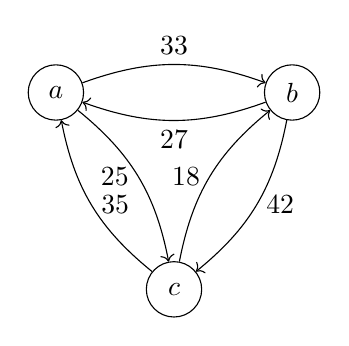
\begin{tikzpicture}[
        vertex/.style={circle, draw, minimum size=20pt, inner sep=0pt},
        every edge/.style={draw, ->, thick},
        bend angle=20
    ]
        \node[vertex] (a) at (0, 0) {$a$};
        \node[vertex] (b) at (3, 0) {$b$};
        \node[vertex] (c) at (1.5, -2.5) {$c$};

        \draw[->] (a) to[bend left] node[above] {$33$} (b);
        \draw[->] (b) to[bend left] node[below] {$27$} (a);

        \draw[->] (a) to[bend left] node[left] {$25$} (c);
        \draw[->] (c) to[bend left] node[right] {$35$} (a);

        \draw[->] (b) to[bend left] node[right] {$42$} (c);
        \draw[->] (c) to[bend left] node[left] {$18$} (b);
    \end{tikzpicture}
    \end{center}

    % Margin Graph
    \begin{center}
    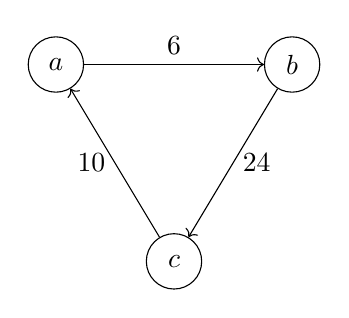
\begin{tikzpicture}[
        vertex/.style={circle, draw, minimum size=20pt, inner sep=0pt},
        every edge/.style={draw, ->, thick}
    ]
        \node[vertex] (a) at (0, 0) {$a$};
        \node[vertex] (b) at (3, 0) {$b$};
        \node[vertex] (c) at (1.5, -2.5) {$c$};

        \draw[->] (a) -- node[above] {$6$} (b);
        \draw[->] (c) -- node[left] {$10$} (a);
        \draw[->] (b) -- node[right] {$24$} (c);
    \end{tikzpicture}
    \end{center}

    We look at the C2 graph, 
    and notice that the 
    \emph{ideal} majority 
    score (when we disregard the acyclicity condition)
    is given by 
    $33 + 42 + 35 = 110$.

    We can consider the 
    linear order 
    $a \succ b \succ c$,
    and observe (via the margin graph)
    that this incurs a penalty of 
    $10$ for the edge $a \succ c$.
    It is not too hard to see, that this means that 
    we get the Kemeny-Score of $110 - 10 = 100$ for this linear order.
    Perhaps, it is not too much of a stretch to notice that 
    this is not the 
    highest Kemeny-Score we can get,
    since we can instead incur the 
    $6$ penalty for the edge $a \succ b$ by considering the linear order
    $b \succ c \succ a$.
\end{example}

\begin{remark}
    We can then reduce the 
    problem of computing the Kemeny winners, 
    to a problem in the 
    margin graph. 
    Namely, 
    we find sets of edges
    that are minimal in total weight, 
    and such that the graph produced 
    by reversing these edges (and keeping the 
    rest of the margin graph as is) is acyclic.
\end{remark}

\begin{idea}
    This idea of picking a subset of edges, reversing the 
    direction of that subset, and then checking 
    acyclicity of the resulting graph, is 
    a little bit of a pain to think about.
    Instead, we would like to think about deleting these edges instead,
    and the following lemma helps with this.
\end{idea}

\begin{lemma}\label{l:inversion-to-deletion}
    Let $G = (V, E)$ be a directed graph, 
    and $E' \subseteq E$ be a subset of edges.
    Then, 
    $G$ can be made acyclic by inverting 
    a subset $E'' \subseteq E'$
    iff
    $(V, E \setminus E')$ is acyclic.
\end{lemma}

\begin{proof}
    \leavevmode \\
    ${\implies}$:
    Easy, remove all of $E'$.

    ${\impliedby}$:
    Greedily insert edges in $E'$ back in,
    one after another. At each step orient the 
    edges so that no cycle forms. If at any stage, 
    both orientations yield a cycle, 
    then the previous graph was cyclic. 
    Contradiction.
\end{proof}

\begin{comment}
    This formulation is not as clean as we may hope, 
    but is necessary, for example, consider the 
    three cycle graph, deleting the whole cycle makes is 
    acyclic, but reversing it does not.
\end{comment}

\begin{remark}
    This lemma, allows us to consider the problem now
    to be, 
    find a subset of edges $E'$ with minimal total weight,
    such that $(V, E \setminus E')$ is acyclic.

    We might hope this to now be rather easy, 
    ``For each cycle, remove the minimum weight edge.'', 
    but cycles may overlap, and so this is slightly more tricky.
\end{remark}

\begin{comment}
    Recall, we showed that 
    reinforcement is satisfied by all 
    scoring rules, and no Condorcet extensions
    --- redefining these properties for 
    SPFs, we can show that there is a 
    Condorcet extension that satisfies reinforcement, 
    namely, Kemeny's rule (cheating, of course by redefining the properties in this context).
\end{comment}

\begin{definition}[Young's Characterization]
    \leavevmode \\
    An SPF $h$ satisfies \emph{reinforcement} if
    for all 
    disjoint sets of voters $N$ and $N'$,
    and all profiles $R_N \in \mathcal{L}(U)^N$ and $R_{N'} \in \mathcal{L}(U)^{N'}$,
    where $h(R_N) \cap h(R_{N'}) \neq \emptyset$,
    then $h(R_N \cup R_{N'}) = h(R_N) \cap h(R_{N'})$
    \footnote{Again, formally, we are considering this notion of an expanded domain.}.
    
    Two alternatives $x$ and $y$ are \emph{adjacent}
    in a preference relation $\gtrsim$ if there is no alternative 
    $z$ such that $x \succ z \succ y$ or $y \succ z \succ x$.
    We say an SPF $h$ satisfies \emph{Condorcet-consistency} if 
    for all profiles $R_N$, 
    $\gtrsim \in h(R_N)$, and $x \succ y$ where $x$ and $y$ are 
    adjacent in $\gtrsim$, we have $x \succ_M y$.
    Moreover, 
    $x \sim_M y$ implies $(\gtrsim \setminus \set{\langle x, y \rangle}) \cup \set{\langle y, x \rangle} \in h(R_N)$
    \footnote{This final condition on $x \sim_M y$ is more of a technicality which says that 
    if there is a tie and one of the linear orders given by 
    $h$ has $x \succ y$, then we can flip the order of $x$ and $y$ in that linear order and it will still be given by $h$.}.
\end{definition}

\begin{remark}
    Consider that Condorcet-consistency, implies the 
    natural notion that we might think of as a Condorcet extension in the 
    context of SPFs. Namely, 
    if there is a Condorcet winner and an SPF is 
    Condorcet-consistent, then the Condorcet winner is ranked above all other alternatives in every linear order given by the SPF.
    \unclear{Why?}
\end{remark}

\begin{theorem}[Young and Levenglick, 1978]
    Kemeny's Rule is the only 
    neutral SPF satisfying 
    reinforcement and Condorcet-consistency.
\end{theorem}

\begin{remark}
    Without going into the proof of the 
    \emph{only} part of the above theorem, 
    it is a good exercise to think why 
    Kemeny's rule is neutral and satisfies reinforcement and Condorcet-consistency.
\end{remark}

\begin{comment}
    Often, we want to reason in 
    the course about profiles by way of their 
    C1, C2, or margin graphs.
    It is often easier to go straight from a graph, 
    and we may not first want to construct 
    a profile which yields 
    that graph.
\end{comment}

\begin{theorem}[McGarvey's Theorem]
    For tournament $G = (V, E)$, 
    there exists a preference profile 
    $R_N$ such that the C1 graph with respect to $R_N$ is $G$.
    Further, the same profile yields a margin graph (the same graph)
    with edge weights of $1$.
\end{theorem}
\begin{proof}
    \unclear{TODO}
\end{proof}

\begin{definition}[Feedback Arc Set]
    The problem 
    \emph{Feedback Arc Set} (FAS)
    is the problem:
    is it possible to make a directed graph acyclic by 
    removing $k$ edges.
\end{definition}

\begin{theorem}
    FAS is NP-Complete (Karp, 1972).
    FAS is NP-Complete when 
    restricted to 
    tournament graphs (Alon, 2006; Charbit et al. 2007; Conitzer 2006), 
    refer to this problem as \textbf{T-FAS}.
\end{theorem}

\begin{theorem}[Bartholdi et al., 1989]
    Deciding whether a 
    there exists a 
    ranking with Kemeny score at least $s$ is 
    NP-Complete.
\end{theorem}
\begin{proof}
    Slightly tricky reduction from T-FAS using McGarvey's theorem
    and Lemma~\ref{l:inversion-to-deletion}.
    Exercise.
\end{proof}

\begin{remark}
    The Kemeny score problem is 
    at least as hard as T-FAS.
    Finding a Kemeny ranking is 
    at least as hard as the Kemeny score problem, 
    so finding a Kemeny ranking is NP-Hard.
    Finding a Kemeny ranking is NP-Hard in the restricted case 
    for even $n \geq 4$ and odd $n \geq 7$.
    If it is NP-Hard to find a Kemeny ranking for $n = 3, 5$ is open.
    Deciding if a given ranking is a Kemeny ranking is 
    CoNP-Complete (clearly).
    There are approximation algorithms for 
    finding a Kemeny ranking.
\end{remark}

\chapter{Weighted Tournament Solutions}

\begin{comment}
    In this chapter, 
    we consider 
    C2 social choice functions.
\end{comment}

\begin{notation}
    Given a preference profile $R_N$,
    and alternatives $x, y \in U$,
    let $m(x, y) := n_{xy} - n_{yx}$ be the majority margin between $x$ and $y$.
    Clearly $m(x, y) = - m(y, x)$, and $m(x, x) = 0$.
\end{notation}

\begin{definition}[Weighted Tournament Solution]
    An SCF is a \emph{weighted tournament 
    solution} if it only depends on 
    $\big(m(x, y)\big)_{x, y \in U}$.
    Often, all we need is the order 
    among $\big(m(x, y)\big)_{x, y \in U}$ (note, this is not 
    the case for Kemeny). Basically, this is the same as 
    be a function of 
    the margin graph.
\end{definition}

\begin{theorem}[Debord's Theorem]
    The following generalises 
    McGarvey's Theorem.


    Let $\big(m(x, y)\big)_{x, y \in U}$ be a collection of 
    integers with 
    $m(x, y) = - m(y, x)$ for all $x, y \in U$,
    and $m(x, x) = 0$ for all $x \in U$.
    Then, there exists a preference profile $R_N$ with majority margins
    $\big(m(x, y)\big)_{x, y \in U}$ if and only if 
    for all $x \neq y$, $m(x, y)$ has the same parity.

    The parity condition makes sense, consider first that 
    $n_{xy} + n_{yx} = n$ 
    and so $m(x, y) = n_{xy} - n_{yx} = 2n_{xy} - n$, 
    which has the same parity as $n$.
\end{theorem}
\begin{proof}
    Exercise.
\end{proof}

\section{Clones}

\begin{example}
    In 1969, Thunder Bay, Ontario, Canada, 
    held a plurality referendum to decide its name.
    \begin{itemize}
        \item Thunder Bay: 15,870 votes
        \item Lakehead: 15,302 votes
        \item The Lakehead: 8,377 votes
    \end{itemize}
    This phenomena is vote splitting, or 
    manipulation by cloning.

    Plurality is especially, susceptible to this, 
    something like instant run-off would
    not fall to this so easily.
\end{example}

\begin{definition}[Clones]
    For a preference profile $R_N$ a 
    subset $C \subseteq U$, s.t. $|U| > |C| \geq 2$ is a set of 
    \emph{clones} if for all 
    $c, c' \in C$, $x \in U \setminus C$, and $i \in N$ it holds that 
    $c \succ_i x$ iff $c' \succ_i x$.

    Informally, a set of clones are always ranked next to each other by every voter, 
    though the ranking among the clones may be arbitrary (clones appear as a contiguous interval in 
    each voters preference relation).
\end{definition}

\begin{observation}[Tideman, 1987]
    Most SCFs are susceptible to manipulation by 
    adding or deleting clones.
\end{observation}

\begin{definition}[Independence of Clones]
    An SCF $f$ satisfies 
    \emph{independence of clones} (IoC)
    if for all profiles $R_N$, 
    feasible set $A \in \mathcal{F}(U)$, and set of clones $C \subseteq A$,
    and $c \in C$ the following two properties hold.

    \begin{enumerate}
        \item 
        For all $a \in A \setminus C$:
        $a \in f(R_N, A) \iff a \in f(R_N, A \setminus \{c\})$.

        \item
        $C \cap f(R_N, A) \neq \emptyset$
        if and only if 
        $C \cap f(R_N, A \setminus \{c\}) \neq \emptyset$.
    \end{enumerate}
    The first property says that 
    adding or removing a clone alternative should 
    not affect the whether a non-clone is 
    selected or not.

    The second says that adding or removing a clone from a clone
    group does not affect whether or not the clone group contains a winner 
    (note we specify clone groups of size at least 2).
\end{definition}

\begin{example}
    Instant-runoff satisfies 
    independence of clones, 
    but we are not too fond of it because it fails to satisfy 
    many other desirable properties:
    it is not monotonic, nor \emph{Condorcet consistent}.
\end{example}

\section{Ranked Pairs}

\begin{definition}[Ranked Pairs: Tideman, 1987]
    The SCF \emph{Ranked Pairs}
    was proposed to achieve independence of clones.
    It may be viewed as a greedy heuristic for finding 
    rankings with a high Kemeny score.

    Ranked Pairs is an SCF that follows more algorithmcally.

    \begin{enumerate}
        \item 
        Order the edges of the majority graph by decreasing weight, 
        use a tiebreaker if necessary (often we assume 
        that their are no ties and also there are no majority ties so 
        that there is an edge between every pair in the majority graph).
        Restrict to just the edges with both endpoints in the feasible set $A$.

        \item
        Initialize an empty graph $G$ on the vertex set of all 
        feasible alternatives $A$.

        \item Process the edges as follows in the order given by
        (1). If $\langle a, b \rangle$ is the next majority edge to be processed:
        \begin{itemize}
            \item  If $G \cup \set{\langle a, b \rangle}$ is acyclic, add $\langle a, b \rangle$ to $G$.
            \item Otherwise, skip $\langle a, b \rangle$ (Alternatively, add $\langle b, a \rangle$ to $G$).
        \end{itemize}
    \end{enumerate}
    This gives a linear order on the feasible alternatives.
    Finally, return the highest ranked alternative in this order, 
    \emph{the ranked pairs winner}.

    Clearly, this is polynomial-time.
    Essentially we are greedily adding edges where we can starting with the ones that give the 
    highest greedy Kemeny score (may not be optimal).
\end{definition}
\unclear{Why does this algorithm always output something?}

\begin{theorem}[Tideman and Zavist, 1989]
    When equipped with a suitable tiebreaker, 
    Ranked Pair satisfies 
    IoC
    \footnote{Caveat: The tiebreaker violates neutrality and/or anonymity}.

    Given a tiebreaker, Ranked Pairs is a 
    resolute SCF and can be computed in polynomial-time.
\end{theorem}

\begin{definition}[PUT Ranked Pairs]
    Parallel-Universes Tiebreaking.
    The irresolute SCF that outputs all alternatives that 
    can win under some tiebreaker, 
    we then can maintain anonymity and neutrality 
    (but annoyingly, does nto satisfy independence of clones).
    Computing it is NP-Hard (reduction from SAT).
\end{definition}

\begin{definition}[Stability for Winners: Holliday and Pacuit, 2023]
    An SCF satisfies
    \emph{stability for winners} if for all profiles $R_N$,
    and all feasible sets $A$ and $b \in U \setminus A$:
    if $a \in f(R_N, A)$ and $a \succ_M b$, then $a \in f(R_N, A \cup \{b\})$.
\end{definition}

\begin{remark}
    Stability for winners implies that there can not be 
    a \emph{spoiler effect} as in 
    the Gore, Bush, Nader case.
\end{remark}




\begin{example}[Ranked Pairs Fails Stability for Winners]
    
    \begin{figure}[H]
    \centering
    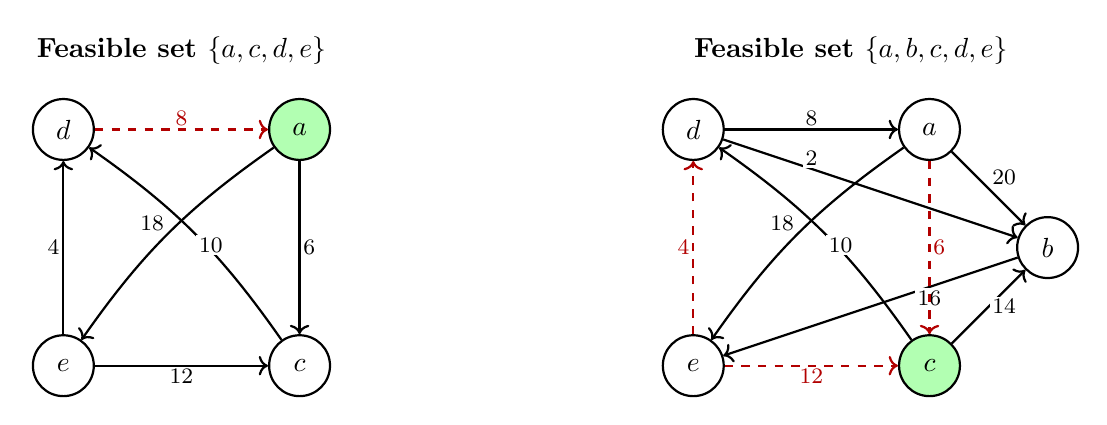
\begin{tikzpicture}[
        vertex/.style={circle, draw, thick, minimum size=22pt, inner sep=0pt},
        winner/.style={vertex, fill=green!30},
        locked/.style={->, thick},
        rej/.style={->, thick, dashed, red!70!black},
        lbl/.style={font=\footnotesize, fill=white, inner sep=1pt}
    ]

    % LEFT GRAPH
    \begin{scope}
        \node at (1.5, 4) {\textbf{Feasible set $\{a, c, d, e\}$}};
        \node[vertex] (d) at (0, 3) {$d$};
        \node[winner] (a) at (3, 3) {$a$};
        \node[vertex] (e) at (0, 0) {$e$};
        \node[vertex] (c) at (3, 0) {$c$};

        \draw[rej] (d) -- node[lbl, above] {$8$} (a);
        \draw[locked] (a) to[bend right=10] 
            node[lbl, above left] {$18$} (e);
        \draw[locked] (e) -- node[lbl, left] {$4$} (d);
        \draw[locked] (a) -- node[lbl, right] {$6$} (c);
        \draw[locked] (e) -- node[lbl, below] {$12$} (c);
        \draw[locked] (c) to[bend right=10] 
            node[lbl, below right] {$10$} (d);
    \end{scope}

    % RIGHT GRAPH
    \begin{scope}[xshift=8cm]
        \node at (2, 4) {\textbf{Feasible set $\{a, b, c, d, e\}$}};
        \node[vertex] (d) at (0, 3) {$d$};
        \node[vertex] (a) at (3, 3) {$a$};
        \node[vertex] (e) at (0, 0) {$e$};
        \node[winner] (c) at (3, 0) {$c$};
        \node[vertex] (b) at (4.5, 1.5) {$b$};

        % Locked edges
        \draw[locked] (a) -- node[lbl, above right] {$20$} (b);
        \draw[locked] (a) to[bend right=10] 
            node[lbl, above left] {$18$} (e);
        \draw[locked] (c) -- node[lbl, right] {$14$} (b);
        \draw[locked] (d) -- node[lbl, above, pos=0.3] {$2$} (b);
        \draw[locked] (b) -- node[lbl, below, pos=0.3] {$16$} (e);
        \draw[locked] (d) -- node[lbl, above] {$8$} (a);
        \draw[locked] (c) to[bend right=10] 
            node[lbl, below right] {$10$} (d);

        % Rejected edges
        
        \draw[rej] (e) -- node[lbl, left] {$4$} (d);
        \draw[rej] (e) -- node[lbl, below] {$12$} (c);
        \draw[rej] (a) -- node[lbl, right] {$6$} (c);
    \end{scope}

    \end{tikzpicture}
    \caption{Ranked Pairs fails stability for winners. 
    Solid arrows are the majority
    edges that are included in the ranked pairs algorithm; 
    dashed red arrows are rejected edges (would create a cycle). 
    Winner shown in green.
    Removing non-winner $b$ changes the winner from $c$ to $a$.}
    \end{figure}
\end{example}

\begin{definition}[The (strong) no show paradox]
    Consider the following situation.
    A profile $R_N$ has that 
    $x$ is a winner under $f$.
    A voter $i \notin N$ ranks $x$ first.
    The new profile
    $R_{N \cup \{i\}}$ no longer gives that $x$ is the winner.

    It is a different type of manipulability, where it would be beneficial
    for a voter to not participate in an election.

    This is known as the \emph{(strong) no show paradox}.
\end{definition}

\begin{example}[Ranked pairs is susceptible to the no show paradox]
    Consider the following 
    margin graph.
    \begin{center}
    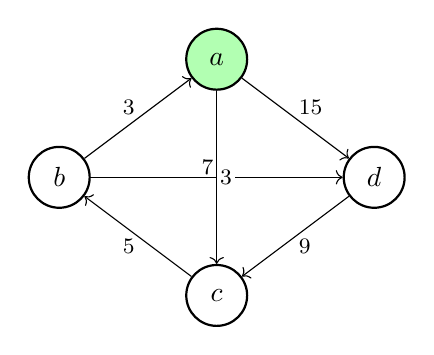
\begin{tikzpicture}[
        vertex/.style={circle, draw, thick, minimum size=22pt, inner sep=0pt},
        winner/.style={vertex, fill=green!30},
        every edge/.style={draw, ->, thick},
        lbl/.style={font=\footnotesize, fill=white, inner sep=1pt}
    ]
        \node[winner] (a) at (2, 3) {$a$};
        \node[vertex] (b) at (0, 1.5) {$b$};
        \node[vertex] (d) at (4, 1.5) {$d$};
        \node[vertex] (c) at (2, 0) {$c$};

        \draw[->] (b) -- node[lbl, above left] {$3$} (a);
        \draw[->] (a) -- node[lbl, above right] {$15$} (d);
        \draw[->] (b) -- node[lbl, above left] {$7$} (d);
        \draw[->] (a) -- node[lbl, right] {$3$} (c);
        \draw[->] (c) -- node[lbl, below left] {$5$} (b);
        \draw[->] (d) -- node[lbl, below right] {$9$} (c);
    \end{tikzpicture}
    \end{center}
    The ranked pairs algorithm will select all but the 
    two $3$ edges, and give that 
    $a$ is the winner.

    Consider the profile now with a new voter $i$
    with preference relation 
    $a \succ_i b \succ_i c \succ_i d$.

    The new profile looks like,
    \begin{center}
    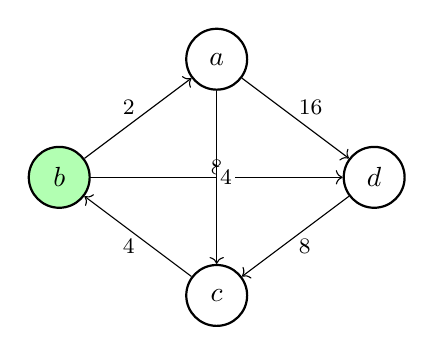
\begin{tikzpicture}[
        vertex/.style={circle, draw, thick, minimum size=22pt, inner sep=0pt},
        winner/.style={vertex, fill=green!30},
        every edge/.style={draw, ->, thick},
        lbl/.style={font=\footnotesize, fill=white, inner sep=1pt}
    ]
        \node[vertex] (a) at (2, 3) {$a$};
        \node[winner] (b) at (0, 1.5) {$b$};
        \node[vertex] (d) at (4, 1.5) {$d$};
        \node[vertex] (c) at (2, 0) {$c$};

        \draw[->] (b) -- node[lbl, above left] {$2$} (a);
        \draw[->] (a) -- node[lbl, above right] {$16$} (d);
        \draw[->] (b) -- node[lbl, above] {$8$} (d);
        \draw[->] (a) -- node[lbl, right] {$4$} (c);
        \draw[->] (c) -- node[lbl, below left] {$4$} (b);
        \draw[->] (d) -- node[lbl, below right] {$8$} (c);
    \end{tikzpicture}
    \end{center}
    And we have winner, $b$.
\end{example}

\begin{definition}[Positive Involvement]
    An SCF $f$ satisfies positive 
    involvement if for all feasible 
    sets $A$ and alternatives $x \in A$,
    and all profiles $R_N$ and $R_{N'}$ where $N' = N \cup \{i\}$, 
    where $\operatorname{Max}(\gtrsim_i, A) = x$: if $x \in f(R_N, A)$, then $x \in f(R_{N'}, A)$.
\end{definition}


\section{Split Cycle}

\begin{definition}
    Consider a preference profile 
    and let $C = (x_1, \dots, x_k)$ be a 
    simple cycle in the margin graph \footnote{A path as opposed to a walk.}, 
    when restricted to a feasible set $A$.
    The splitting number 
    $\operatorname{sp}(C)$ is the smallest margin between 
    consecutive alternatives in $C$.

    We say that $a$ \emph{defeats} $b$ if 
    $a \succ_M b$ and for every (simple) cycle $C$ containing $a$ and $b$,
    $\operatorname{sp}(C) < m(a, b)$.

    Informally, we think that $a$ defeats $b$ if 
    it wins it strictly wins in the majority relation, and 
    further the edge from $a \to  b$  is never the weakest link on a cycle.
\end{definition}

\begin{definition}[Split Cycle]
    The social choice function 
    \emph{Split Cycle} is the function that returns 
    all undefeated candidates.

    Denote it by $f_{\text{SC}}$.

    We can think of the computation of split cycle as simply 
    starting with the margin graph, identifying every simple cycle in the 
    margin graph and deleting the lightest edge along each cycle, 
    finally it outputs those alternatives with no incoming edges exactly.
\end{definition}

\begin{example}
    Consider the following margin graph,
    in colours each simple cycle is highlighted. 
    The Split Cycle algorithm would remove those 
    edges corresponding to the 
    lightest 
    weight in the cycle, 
    and then output the
    candidates that have no incoming edges --- these are 
    precisely the 
    undefeated candidates.
    The remaining edges give exactly the 
    defeat relation.

    \begin{figure}[H]
    \centering
    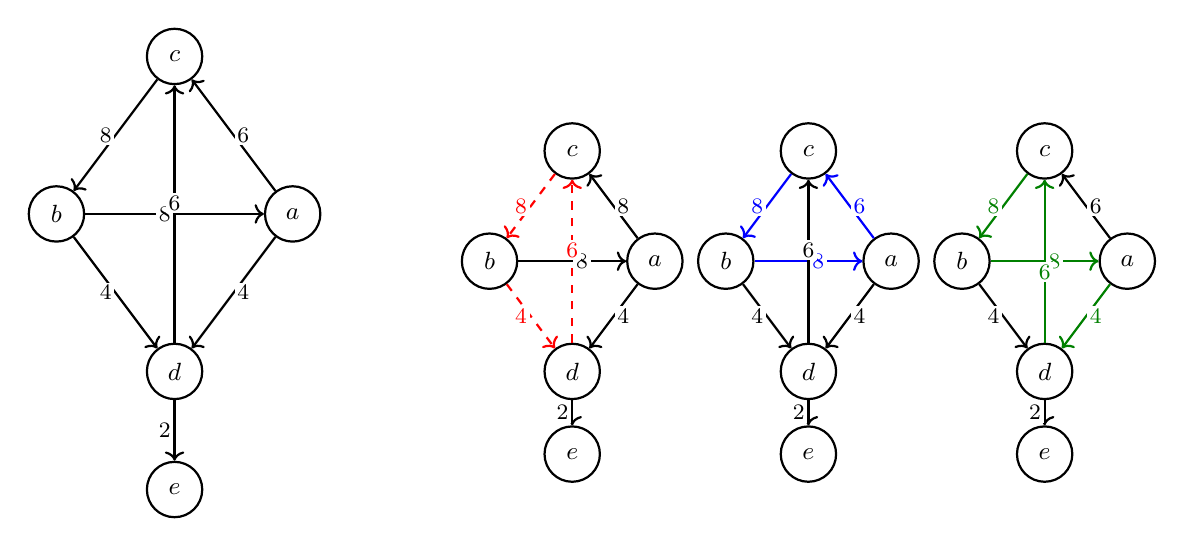
\begin{tikzpicture}[
        vertex/.style={circle, draw, thick, minimum size=20pt, inner sep=0pt, font=\small},
        arr/.style={->, thick},
        lbl/.style={font=\footnotesize, fill=white, inner sep=1pt}
    ]

    % ---- MAIN GRAPH ----
    \begin{scope}
        \node[vertex] (c) at (1.5, 4) {$c$};
        \node[vertex] (b) at (0, 2) {$b$};
        \node[vertex] (a) at (3, 2) {$a$};
        \node[vertex] (d) at (1.5, 0) {$d$};
        \node[vertex] (e) at (1.5, -1.5) {$e$};

        \draw[arr] (c) -- node[lbl, left] {$8$} (b);
        \draw[arr] (a) -- node[lbl, right] {$6$} (c);
        \draw[arr] (b) -- node[lbl, left] {$8$} (a);
        \draw[arr] (b) -- node[lbl, left] {$4$} (d);
        \draw[arr] (a) -- node[lbl, right] {$4$} (d);
        \draw[arr] (d) -- node[lbl, above] {$6$} (c);
        \draw[arr] (d) -- node[lbl, left] {$2$} (e);
    \end{scope}

    % ---- RED CYCLE: (c, b, d) ----
    \begin{scope}[xshift=5.5cm, scale=0.7]
        \node[vertex] (c) at (1.5, 4) {$c$};
        \node[vertex] (b) at (0, 2) {$b$};
        \node[vertex] (a) at (3, 2) {$a$};
        \node[vertex] (d) at (1.5, 0) {$d$};
        \node[vertex] (e) at (1.5, -1.5) {$e$};

        \draw[arr, red, dashed] (c) -- node[lbl, left, text=red] {$8$} (b);
        \draw[arr] (a) -- node[lbl, right] {$8$} (c);
        \draw[arr] (b) -- node[lbl, right] {$8$} (a);
        \draw[arr, red, dashed] (b) -- node[lbl, left, text=red] {$4$} (d);
        \draw[arr] (a) -- node[lbl, right] {$4$} (d);
        \draw[arr, red, dashed] (d) -- node[lbl, above, text=red] {$6$} (c);
        \draw[arr] (d) -- node[lbl, left] {$2$} (e);
    \end{scope}

    % ---- BLUE CYCLE: (c, b, a) ----
    \begin{scope}[xshift=8.5cm, scale=0.7]
        \node[vertex] (c) at (1.5, 4) {$c$};
        \node[vertex] (b) at (0, 2) {$b$};
        \node[vertex] (a) at (3, 2) {$a$};
        \node[vertex] (d) at (1.5, 0) {$d$};
        \node[vertex] (e) at (1.5, -1.5) {$e$};

        \draw[arr, blue] (c) -- node[lbl, left, text=blue] {$8$} (b);
        \draw[arr, blue] (a) -- node[lbl, right, text=blue] {$6$} (c);
        \draw[arr, blue] (b) -- node[lbl, right, text=blue] {$8$} (a);
        \draw[arr] (b) -- node[lbl, left] {$4$} (d);
        \draw[arr] (a) -- node[lbl, right] {$4$} (d);
        \draw[arr] (d) -- node[lbl, above] {$6$} (c);
        \draw[arr] (d) -- node[lbl, left] {$2$} (e);
    \end{scope}

    % ---- GREEN CYCLE: (c, b, a, d) ----
    \begin{scope}[xshift=11.5cm, scale=0.7]
        \node[vertex] (c) at (1.5, 4) {$c$};
        \node[vertex] (b) at (0, 2) {$b$};
        \node[vertex] (a) at (3, 2) {$a$};
        \node[vertex] (d) at (1.5, 0) {$d$};
        \node[vertex] (e) at (1.5, -1.5) {$e$};

        \draw[arr, green!50!black] (c) -- node[lbl, left, text=green!50!black] {$8$} (b);
        \draw[arr] (a) -- node[lbl, right] {$6$} (c);
        \draw[arr, green!50!black] (b) -- node[lbl, right, text=green!50!black] {$8$} (a);
        \draw[arr] (b) -- node[lbl, left] {$4$} (d);
        \draw[arr, green!50!black] (a) -- node[lbl, right, text=green!50!black] {$4$} (d);
        \draw[arr, green!50!black] (d) -- node[lbl, below, text=green!50!black] {$6$} (c);
        \draw[arr] (d) -- node[lbl, left] {$2$} (e);
    \end{scope}

    \end{tikzpicture}

    \vspace{0.5em}
    \begin{tabular}{lll}
        \textcolor{red}{Red: cycle $(c, b, d)$, $\operatorname{sp} = 4$} &
        \textcolor{blue}{Blue: cycle $(c, b, a)$, $\operatorname{sp} = 6$} &
        \textcolor{green!50!black}{Green: cycle $(c, b, a, d)$, $\operatorname{sp} = 4$}
    \end{tabular}
    \end{figure}

    It is clear, that the defeat relation is 
    \textbf{not} transitive, since after deleting these three 
    lightest edges, $c$ defeats $b$ and 
    $b$ defeats $a$, but $c$ does not defeat $a$.

\end{example}

\begin{lemma}[Defeat Relation is acyclic]
    We can think of \emph{defeat} as a relation on alternatives.
    To show that 
    Split Cycle gives a non-empty 
    choice set, it suffices
    (but is not necessary) to show that
    the defeat relation is acyclic.
\end{lemma}
\begin{proof}
    Suppose for contradiction that 
    there is a cycle under the defeat relation,
    then there is a 
    simple cycle under the 
    the defeat relation, say 
    $a_1, \dots, a_k$.
    Then, by definition of the defeat relation,
    $C := a_1, \dots, a_k$ is a simple cycle in the 
    margin graph.
    Then, consider that 
    for each edge $a_i \to a_{i+1}$ (incl. the edge $a_k \to a_1$),
    in the defeat cycle, 
    by definition of defeat, we have that $m(a_i, a_{i+1}) > \operatorname{sp}(C)$.
    Consider that by definition of splitting number, there is some edge $a_j \to a_{j+1}$ in $C$ such that
    $m(a_j, a_{j+1}) = \operatorname{sp}(C)$, contradicting 
    the fact that $m(a_j, a_{j+1}) > \operatorname{sp}(C)$.
\end{proof}

\begin{observation}
    To check whether 
    $a$ defeats $b$, we only need to check the simple cycles containing 
    the edge $a \to b$. 
    That is we need not check 
    cycles containing 
    $a$ and $b$ when they are not adjacent, and certainly not 
    all simple cycles in the margin graph. We omit proof.
\end{observation}

\begin{definition}
    For alternatives $a, b \in U$ with 
    $a \succ_M b$, define the \emph{cycle number} to be 
    \[
        \operatorname{cyc}(a, b) := \max \bigg(\set{0} \cup
            \set{\operatorname{sp}(C) :  \text{C a simple cycle in margin graph 
            containing edge} \langle a, b \rangle}
        \bigg)
    \]

    Informally, 
    the cycle number of $a$ and $b$ is the
    the maximum splitting number among simple cycles containing the edge $a \to b$, 
    or $0$ if there are no such cycles.
\end{definition}

\begin{lemma}
    $a$ defeats $b$ if and only if 
    $m(a, b) > \operatorname{cyc}(a, b)$.
\end{lemma}
\begin{proof}
   Exercise. 
\end{proof}

\begin{remark}
    The naive approach we give to 
    compute $f_{\text{SC}}$ requires checking all 
    simple cycles in the margin graph,
    which is exponential in the number of alternatives.
    We hope to use the above ideas, to get a more computationally
    appealing method to compute 
    $f_{\text{SC}}$.
\end{remark}


\begin{definition}
    The \emph{strength} of a path 
    in the margin graph is the smallest 
    margin between consecutive alternatives on the path.

    Let $\operatorname{strength}(x, y)$ denote the strength of the strongest path 
    from $x$ to $y$.
\end{definition}

\begin{lemma}\label{l:strength-characterization-SC}
    $a$ defeats $b$ if and only if
    $a \succ_M b$ and 
    $\operatorname{strength}(b, a) < m(a, b)$.
\end{lemma}

\begin{remark}
    We characterise the notion of defeat via 
    strength because $\operatorname{strength}(\cdot, \cdot)$ is a notion that \emph{can}
    be computed efficiently using a variant of the 
    Floyd-Warshall algorithm ($O(|A|^3)$).
    Thus, we can compute split cycle winners in polynomial time.
    Explicitly we do this by, 
    \begin{enumerate}
        \item Compute the margin graph from the profile: $O(|A|^2n)$
        \item Compute for each pair of alternatives 
        $\operatorname{strength}(a, b)$: $O(|A|^3)$ each so $O(|A|^5)$ total.
        \item For each pair, check if 
        $a$ defeats $b$ by checking if $a \succ_M b$ and $\operatorname{strength}(a, b) < m(a, b)$: $O(|A|^2)$.
        \item Return all those alternatives with no incoming edges in the defeat graph.
    \end{enumerate}
\end{remark}

\begin{proposition}[Split Cycle satisfies stability for winners]
\end{proposition}
\begin{proof}
    Suppose for contradiction that 
    split cycle fails stability for winners, then there is a profile $R_N$,
    feasible set $A$, and $b \in U \setminus A$ such that there is some 
    $a \in f_{\text{SC}}(R_N, A)$ and $a \succ_M b$, but $a \notin f_{\text{SC}}(R_N, A \cup \{b\})$.

    Consider that adding $b$ to the set of feasible alternatives can only 
    add paths in the margin graph between vertices, 
    so $\operatorname{strength}_{A \cup \set{b}}(x, y) \geq \operatorname{strength}_A(x, y)$
    for all $x, y \in A$.
    For contradiction, suppose
    $a$ is defeated in
    $A \cup \set{b}$, then there is some alternative $c$ such that
    $\operatorname{strength}_{A \cup \set{b}}(a, c) < m(c, a)$.
    But $\operatorname{strength}_{A \cup \set{b}}(a, b) \geq \operatorname{strength}_A(a, b)$, 
    thus $\operatorname{strength}_{A}(a, c) < m(c, a)$.
    If $c \in A$, then $a$ is defeated in $A$, contradicting that $a \in f_{\text{SC}}(R_N, A)$.
    Thus, $c = b$, but this gives a cyclic strict 
    majority between $a$ and $b$, since $a \succ_M b$, giving contradiction.
\end{proof}

\begin{proposition}[Split Cycle satisfies positive involvement]
\end{proposition}
\begin{proof}
    Exercise.
\end{proof}

\begin{proposition}[Split Cycle satisfies independence of clones]
\end{proposition}
\begin{proof}
    Omitted.
\end{proof}

\begin{proposition}[Split Cycle subsumes ranked pairs]
    If $f_{\text{RP}}$ is the ranked pairs SCF, then for all profiles $R_N$ and feasible sets $A$,
    $f_{\text{RP}}(R_N, A) \subseteq f_{\text{SC}}(R_N, A)$.
\end{proposition}

\begin{proof}[Sketch]
    We omit the details of tie-breaking.

    Suppose that $a \notin f_{\text{SC}}(R_N, A)$, then there is some $b$ that defeats $a$.
    Then, Lemma~\ref{l:strength-characterization-SC}'s gives that 
    $b \succ_M a$ or $\operatorname{strength}(b, a) < m(a, b)$.
    Now consider the cycle formed by the traversal 
    from $b \to_M a$ and then along the strongest path from $a$ to $b$.
    At some point the ranked pairs algorithm will 
    encounter the edge 
    $b \to a$ and will add it because, 
    all cycles containing $b \to a$ have splitting number less than $m(a, b)$,
    so the ranked pairs algorithm will never reject the edge $b \to a$, and thus $a$ can not be the winner under ranked pairs.
\end{proof}


\begin{comment}
    To understand the trade-offs between Ranked Pairs and 
    Split Cycle, we briefly look at the following impossibility results.

    First, note that both Ranked Pairs and Split Cycle satisfy
    \emph{ordinal margin invariance}; that is they depend only on the 
    ordering of the margins 
    $(m(x, y))_{x, y \in U}$, not on the actual values of the margins.
    Note, Kemeny does care about the numbers not just their ordering.
\end{comment}

\begin{theorem}[Holliday, 2023]
    The following are incompatible:
    Condorcet extension, 
    Condorcet loser criterion, 
    ordinal margin invariance, 
    positive involvement, and 
    resolvability.

    Where by \emph{Condorcet loser criterion} we mean that we 
    never select a Condorcet loser. 
    And, by \emph{resolvability} we mean that for all profiles $R_N$ and feasible sets $A$,
    when $|f(R_N, A)| > 1$, there is some profile $R_{N \cup \set{i}}$ such that 
    $|f(R_{N \cup \set{i}}, A)| = 1$ (we can always add one voter to break a tie).
\end{theorem}

\begin{remark}
    Split Cycle satisfies all but resolvability,
    while Ranked Pairs satisfies all but positive involvement.
\end{remark}

\begin{definition}[Quasi-Resoluteness]
    An SCF $f$ is \emph{quasi-resolute} if for all profiles $R_N$ and feasible sets $A$,
    where the edges of the margin graph are all 
    distinct, then $|f(R_N, A)| = 1$.

    Such profiles are sometimes called 
    \emph{uniquely weighted}. It is clear that they do not 
    permit majority ties, i.e. for all $x \neq y$, $m(x, y) \neq 0$.
\end{definition}

\begin{theorem}[Holliday et al., 2024]
    There is no anonymous and neutral SCF that 
    satisfies stability for winners and 
    quasi-resoluteness.
\end{theorem}


\chapter{Multiwinner Voting Rules}

\begin{idea}
    What does multiwinner votine mean? So far, 
    we have modelled alternatives as mutually exclusive outcomes, and we 
    wanted to the chose the \emph{best} alternative, or rank all alternatives.
    Of course, many rules we have discussed are irresolute, but this 
    is not exactly desired behavior --- our framework ushered us away from 
    multiple winners (implicitly we imagine some out of framework tie breaker).
    
    What if instead, we imagine we \emph{must} elect a
    a specifically sized ($k$) set of of alternatives.

    In principle, we could model multiwinner elections with the tools we have thus far, 
    we could have voters just rank their preferences where candidates are different 
    $k$-subsets of alternatives (different committees) --- but this gives 
    exponential number of alternatives, and thus is not computationally appealing, nor natural.

    Another idea is to use a 
    social welfare function, and pick the 
    top $k$ alternatives in the social welfare ordering, 
    we revisit this later.
\end{idea}


\begin{remark}
    We consider two 
    different frameworks for 
    multiwinner voting,
    whereby voters \emph{indirectly}
    express preferences over committees.

    \begin{itemize}
        \item The \emph{Apportionment setting}:
        candidates are grouped into 
        \emph{parties} and voters can support a single party only.
        The underlying assumption is that:
        voters only care about how many 
        candidates from their party are selected.

        This models, \emph{party-list election}, which are often used in 
        parliamentary elections.
        Intuitively, it seems clear that it kind of limits the 
        expressive power of voters.


        \item The \emph{Approval-Based setting}, voters 
        can approve whichever candidates, but
        they do not rank them (still less expressive than our 
        previous settings).
        The assumption is that voters only care about how many candidates
        that they approve of are selected.
    \end{itemize}

    In both settings, we are interested in a 
    notion of \emph{proportional representation}.
\end{remark}

\section{Apportionment Setting}

\begin{definition}
    In the apportionment setting,
    we have a set of parties $P = \{P_1, \dots, P_p\}$, and 
    each voter votes for exactly one party. 

    For each party $P_i$ let $v_i$ denote the number of votes it recieves.
    The goal is to allocate a given number of seats among the parties, 
    \emph{proportional} to the votes.

    An instance of the apportionment problem is given by the pair 
    $(\vec{v}, h)$ where $\vec{v} = (v_1, \dots, v_p) \in \mathbb{N}^p$
    is the \emph{vote distribution} and $h \in \mathbb{N}_{>0}$ is the 
    \emph{committee size} or \emph{house size}.

    We denote the total number of votes by 
    $v_+ := \sum_{i=1}^p v_i$.

    The seat distribution is the vector 
    $\vec{x} = (x_1, \dots, x_p) \in \mathbb{N}^p$ where $x_i$ is the number of seats allocated to party $P_i$,
    and $\sum_{i=1}^p x_i = h$.
\end{definition}

\begin{remark}
    An equivalent problem: For each state in a union, 
    allocate a number of seats proportional to the 
    population of the state.
\end{remark}

\begin{example}
    $\vec{v} = (7270, 1230, 220); h = 21$, and a 
    seat distribution (with respect to $\vec{v}$ and $h$) is $\vec{x} = (15, 4, 2)$.
\end{example}

\begin{definition}[Apportionment Method]
    An \emph{apportionment method} $M$ maps 
    every instance $(\vec{v}, h)$ to a non-empty set $M(\vec{v}, h)$ of seat distributions.
\end{definition}

\begin{definition}[Quota]
    Ideally, we would like to give each party its exact \emph{proportional share} of seats.
    For $(\vec{v}, h)$, the \emph{quota} of party $P_i$ is 
    given by 
    \[
        q_i := \frac{v_i}{v_+} \cdot h
    \]
    Of course, this is not in general an integer.

    We call the fraction 
    $\frac{v_+}{h}$ the \emph{Hare quota}, 
    and see that equivalently 
    $
    q_i = \frac{v_i}{\text{Hare quota}}$.
\end{definition}


\begin{definition}[Hamilton Method]
    The \emph{Hamilton method} has two steps.
    \begin{enumerate}
        \item Calculate quotas and give 
        each party $\lfloor q_i \rfloor$ seats.
        (Note, the sum of the floor of these quotas is $\leq h$).

        \item Give the remaining $r$ seats (if any) to each 
        of the $r$ parties with the largest fractional part of their quota (
            largest $q_i - \lfloor q_i \rfloor$
        ).

    \end{enumerate}
\end{definition}

\begin{definition}[D'Hont Method]
    Find an integer divisor $d$, such that 
    \[
        \sum_{i=1}^p \left\lfloor \frac{v_i}{d} \right\rfloor = h
    \]
    Then, we give party $P_i$ $\left\lfloor \frac{v_i}{d} \right\rfloor$ seats.

    Such a divisor always exists
    when the number of votes for each party are 
    pairwise distinct, and while it need not exist uniquely,
    it always apportions the same seat distribution.
\end{definition}

\begin{remark}
    The seat distribution found by 
    the D'Hont method can be constructed by the following method.

    \begin{itemize}
        \item Define the $j$-th divisor as 
        $d(j) = j$
        \item Construct the table with numbers $\frac{v_i}{d(j)}$ for $i \in [p]$ and $j \in \mathbb{N}$
        
        \item Choose the largest $h$ entries of this table and 
        distribute seats accordingly
    \end{itemize}

    \begin{figure}[H] 
        \centering
        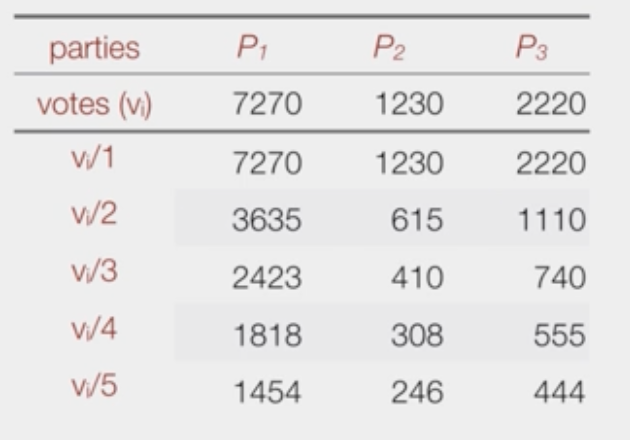
\includegraphics[width=\textwidth]{seq-DHondt.jpg}
        \caption{Sequential D'Hondt method table.}
    \end{figure}


    Why does this work? (Think about it.)
\end{remark}

\begin{remark}
    We can choose the values of 
    the divisors $d(j)$ differently, to get other 
    apportionment methods, known as \emph{divisor methods}.
    For example, the Sainte-Laguë method uses $d(j) = 2j - 1$, 
    which can lead to different distributions.
\end{remark}

\subsection{Axioms for Apportionment Methods}

\begin{definition}[Basic Apportionment Properties]
    \leavevmode \\
    \begin{itemize}
        \item \emph{Impartiality}: the only information that matters is the vote distribution $\vec{v}$ and the house size $h$.
        \item \emph{Exactness}: if all the quotas are integers, then 
        the apportionment method gives each party its quota ($x_i = q_i$).
        \item \emph{Homogeneity}: if all votes are multiplied by the same positive factor,
        the outcomes do not change (the only thing that matters are the quotas).
        \item \emph{Concordance}: a party with strictly more votes than another, 
        cannot be allocated fewer seats than the other, i.e. 
        $v_i > v_j \implies x_i \geq x_j$.
    \end{itemize}

    All the rules we have seen, satisfy these properties, in fact most natural 
    apportionment methods satisfy these properties.
\end{definition}

\begin{idea}
    We will focus on slightly harder 
    properties to satisfy:
    \emph{quota property}, \emph{committee monotonicity}, 
    and \emph{population monotonicity}.
\end{idea}

\subsection{Quota Property}

\begin{definition}[Quota Property]
    An apportionment method $M$ satisfies the
    \emph{quota property} if for all instances $(\vec{v}, h)$,
    for all $x \in M(\vec{v}, h)$, 
    $x_i \in \{\lfloor q_i \rfloor, \lceil q_i \rceil\}$.
\end{definition}

\begin{example}
    \leavevmode \\
    \begin{itemize}
        \item The Hamilton method satisfies the quota property (reason why?).
        \item The D'Hondt method does not satisfy the quota property, 
        see the following example.
        \begin{center}
        \begin{tabular}{c c c c}
            \hline
            party & $P_1$ & $P_2$ & $P_3$ \\
            \hline
            votes ($v_i$) & 7270 & 1230 & 2220 \\
            quota ($q_i$) & 14.92 & 2.52 & 4.56 \\
            seats ($x_i$) & 16 & 2 & 4 \\
            \hline
            \multicolumn{4}{c}{$h = 22$}
        \end{tabular}
        \end{center}
    \end{itemize}
\end{example}

\begin{definition}[Lower Quota]
    The weaker axiom 
    \emph{lower quota} requires that
    for all instances $(\vec{v}, h)$, for all $x \in M(\vec{v}, h)$,
    $x_i \geq \lfloor q_i \rfloor$.
\end{definition}

\begin{theorem}[Balinski and Young, 1982]
    D'Hondt's method satisfies 
    the lower quota property.
    Moreover, it is the only 
    divisor method that satisfies the lower quota property.
\end{theorem}


\subsection{Committee Monotonicity}

\begin{example}[The Alabama Paradox]
    Increasing the committee size may result in some 
    party having fewer seats.

    \begin{center}
    \begin{tabular}{c c c c}
        \hline
        party & $P_1$ & $P_2$ & $P_3$ \\
        \hline
        votes ($v_i$) & 7270 & 1230 & 2220 \\
        quota ($q_i$) & 14.24 & 2.41 & 4.35 \\
        seats ($x_i$) & \textbf{14} & \textbf{3} & \textbf{4} \\
        \hline
        \multicolumn{4}{c}{$h = 21$}
    \end{tabular}
    \quad $\to$ \quad
    \begin{tabular}{c c c c}
        \hline
        party & $P_1$ & $P_2$ & $P_3$ \\
        \hline
        votes ($v_i$) & 7270 & 1230 & 2220 \\
        quota ($q_i$) & 14.92 & 2.52 & 4.56 \\
        seats ($x_i$) & \textbf{15} & \textbf{2} & \textbf{5} \\
        \hline
        \multicolumn{4}{c}{$h = 22$}
    \end{tabular}
    \end{center}
\end{example}

\begin{definition}[Committee Monotonicity]
    An apportionment method $M$ satisfies \emph{committee monotonicity}
    if this can never happen.
\end{definition}

\begin{example}
    The Hamilton method fails committee monotonicity (see the above example),
    but the D'Hondt method satisfies committee monotonicity,
    which can be seen by the tabular definition of 
    D'Hondt's method (and likewise for all divisor methods).
\end{example}

\subsection{Population Monotonicity}

\begin{example}[The Population Paradox]
    A party that loses votes may gain seats at the expense of a party that loses votes.
    Formally, 
    there are two vote distributions $\vec{v}$ and $\vec{v}'$ such that,
    \begin{itemize}
        \item $v_i < v_i'$ and $v_j > v_j'$ for some $i \neq j$.
        \item For some $x \in M(\vec{v}, h)$ and $x' \in M(\vec{v}', h)$,
        $x_i > x_i'$ and $x_j < x_j'$.
    \end{itemize}
    That is, we cannot have party $i$ gaining votes and 
    party $j$ losing votes resulting in party $i$ losing seats and party $j$ gaining seats.
\end{example}

\begin{definition}[Population Monotonicity]
    An apportionment method $M$ satisfies \emph{population monotonicity} if this can never happen.
    Note there are no requirements on 
    the other parties, they can gain or lose votes as they please.
\end{definition}

\begin{example}
    The Hamilton method fails population monotonicity, but the D'Hondt method satisfies it.
\end{example}

\begin{theorem}[Balinski and Young, 1982]
    There is no concordant apportionment method that satisfies both 
    the quota property and population monotonicity.
\end{theorem}

\begin{remark}
    A more natural notion is called \emph{vote monotonicity}, 
    which requires that if a party gains votes (and the rest of the 
    parties recieve the same number of votes), it should not lose seats.

    It is not known, if there is a 
    apportionment method that satisfies the quota property, committee monotonicity, and vote monotonicity
    (open problem).
\end{remark}

\section{Approval-based Multiwinner Voting}

\begin{comment}
    We need to flesh out what is even meant by 
    \emph{proportional representation} in this setting.
\end{comment}

\begin{idea}
    Voters express their preferences with \emph{approval votes}.
    Think of a list of the candidates and each voter puts a 
    checkmark against the ones they approve of, and 
    leaves the rest blank.
\end{idea}

\begin{definition}[Approval-Based Multiwinner Rule]
    Suppose we have a finite set of candidates $C$, 
    and a finite set of voters $N = \{1, \dots, n\}$. 
    We let 
    $A_i \subseteq C$ denote the set of candidates that voter $i$ approves of, 
    note $A_i$ is free to be any subset of $C$.

    A \emph{committee} of size $k$ is a $k$-sized subset of 
    $C$, most often we denote it $W \subset C$.

    Given a \emph{preference profile} 
    $A_N = (A_1, \dots, A_n)$
    (note our notion of preference profile here does \emph{not}
    coincide with our previous notion of preference profile),
    and a committee size $k$, an \emph{approval-based multiwinner rule} is a function
    that maps $(A_N, k)$ to a non-empty set of committees
    \footnote{As usual we map to a set instead of a singleton for reason of symmetry}
    of size $k$.
\end{definition}

\subsection{Approval-based Multiwinner Rules}

\begin{definition}[Approval Voting (AV)]
    The \emph{approval voting} rule,
    computes the number of voters approving each candidate,
    then outputs the $k$ candidates with the most approvals.
\end{definition}

\begin{notation}
    For $c \in C$, let 
    $N_c = \{i \in N : c \in A_i\}$ denote the set of voters that approve of candidate $c$ (\emph{approvers}), 
    and let $n_c = |N_c|$ denote the number of voters that approve of candidate $c$ (\emph{approval score}).
\end{notation}

\begin{example}
    What problems arise from such a system.
    We can consider that there may be an alternatives ranked 
    as having the $k + 1$-th approval scores. In fact such an alternative could be 
    very close to the $k$-th approval score, but it is not selected.
    We aim for some notion of proportional representation, but this 
    doesn't feel particularly proportional.

    For a concrete example suppose:
    $C = \set{a, b, c, x, y}$, $k = 3$, and $|N| = 9$.

    Suppose we have a profile where 
    5 voters approve of $a$, $b$ and $c$ only,
    and 4 voters approve of $x$ and $y$ only.
    Then, $a$, $b$, and $c$ are the winners under approval voting, but
    $x$ and $y$ are not selected, even though they have a very high
    approval score (4 out of 9).

    The above is an example of a 
    \emph{dictatorship of the majority}, where the majority gets all the seats, and the minority gets none.
\end{example}

\begin{definition}[Satisfaction-AV (SAV)]
    The \emph{satisfaction-approval voting} rule, 
    choses committee(s) $W$ that maximize the total satisfaction:
    \[
        \sum_{i \in N} \operatorname{sat}(i, W)
    \]
    Where $\operatorname{sat}(i, W) = \frac{|A_i \cap W|}{|A_i|}$.

    Informally, $\operatorname{sat}(i, W)$
    is the fraction of candidates that voter $i$ approves of that are selected in committee $W$, and 
    we optimise maximising the sum of this quantity over all voters.
\end{definition}

\begin{example}
    In the above example,
    the satisfaction-approval voting rule would select
    all the committees with one 
    candidates from $\{a, b, c\}$ and one candidate from $\{x, y\}$
    (which seems weird).
\end{example}

\begin{remark}
    We can conceptualise 
    SAV by considering each voter having 
    weight $1$ which they distribute equally to 
    the candidates they approve of, and then we select the $k$ candidates with the 
    highest total weight.
\end{remark}

\begin{definition}[Greedy-AV]
    Iteratively construct 
    the committee by at each step adding a candidate that is approved by the 
    most voters that do not yet have a member they approve of in the partially constructed 
    committee.
    
    We say that a voter $i$ is represented in $W$ if 
    $A_i \cap W \neq \emptyset$.
    If / when all voters are represented, we can add any candidates we like to fill up the committee.
\end{definition}

\begin{example}
    In the above example
    the greedy-AV rule would select all the committees with one
    candidates from $\{a, b, c\}$ and one candidate from $\{x, y\}$.
\end{example}

\begin{definition}[Proportional Approval Voting(PAV)]
    Choose committee(s) $W$ maximizing $\operatorname{score}(W) = 
    \sum_{i \in N} \operatorname{score}(i, W)$, where,
    \[
        \operatorname{score}(i, W) = 1 + \frac{1}{2} + \cdots + \frac{1}{|A_i \cap W|}
    \]

    The intuition behind this is that 
    a voter gets diminishingly happy the more of her 
    approved candidates are selected, so we give her a score of $1$ for the first approved candidate selected,
    $\frac{1}{2}$ for the second approved candidate selected, and so on.
\end{definition}

\begin{remark}
    PAV is clearly infeasible to compute, we can 
    construct a greedy version of it that is computable in 
    polynomial time, though it of course, does not give 
    the same outcome as PAV.
\end{remark}

\begin{definition}[Sequential Proportional Approval Voting (seqPAV)]
    We iteratively construct the committee
    by at each step adding a candidate that maximises the increase in the
    PAV score of the committee.
\end{definition}

\begin{algorithm}[H]
\caption{Sequential PAV}
\begin{algorithmic}[1]
\State $W \gets \emptyset$
\While{$|W| < k$}
    \State Select $c^* \in C \setminus W$ maximizing $\operatorname{score}(W \cup \{c^*\})$
    \State $W \gets W \cup \{c^*\}$
\EndWhile
\State \Return $W$
\end{algorithmic}
\end{algorithm}

\begin{definition}[Generalized PAV ($\vec{w}$-PAV)]
    Use PAV with an arbitrary \emph{weight vector}
    $\vec{w} = (w_1, w_2, \dots)$ where $w_j$ is the weight given
    to a voter for having $j$ approved candidates selected in the committee.
    Thus, we maximise 
    \[
        \operatorname{score}_{\vec{w}}(W) = \sum_{i \in N} \operatorname{score}_{\vec{w}}(i, W)
    \]
    Where here $\operatorname{score}_{\vec{w}}(i, W) = w_1 + w_2 + \cdots + w_{|A_i \cap W|}$.
\end{definition}

\begin{remark}
    If we consider the weight vector $\vec{w} = (1, 1, 1, \dots)$, then $\vec{w}$-PAV
    is nothing but Approval Voting.

    For the vector 
    $\vec{w} = (1, 0, 0, \dots)$, we get 
    exactly Greedy-AV.

    Can we make a simillar comment about 
    SAV? Think, why or why not?
\end{remark}

\subsection{Representative Committees}

\begin{idea}
    How do we formalise that a 
    committee is representative of a preference profile?

    Some intuition gives that 
    groupings of size $n / k$ 
    should \emph{have} at least one 
    representative candidate
    (where $n$ is the number of voters and $k$ is the committee size, and 
    $n/k$ is an analog of the Hare quota in the apportionment setting).

    A few problems with this intuition are:
    \begin{itemize}
        \item How do we group the voters into blocks of size $n / k$?
        \item What does it mean for a group of voters to have a representative candidate?
    \end{itemize}

    A first attempt could be the following.
    For any $S \subseteq N$ with $|S| \geq n / k$,
    there should be some candidate $c \in W$ \emph{representing} $S$ ---
    but as mentioned above, what does it mean for $c$ to represent $S$?

    Instead, lets refine this approach.
    Call a voter group $S \subseteq N$ \emph{cohesive} if there is some candidate
    $c$ that all voters in $S$ approve of, i.e. $\bigcap_{i \in S} A_i \neq \emptyset$.
    Then, we can say that a committee is representative if for every cohesive group $S$ with
    $|S| \geq n / k$, there is some candidate in the committee that represents $S$,
    i.e. $\bigcap_{i \in S} A_i \cap W \neq \emptyset$.
    Where here, by represents we mean a candidate approved by all members
    in the cohesive voter group.
\end{idea}

\begin{example}
    Unfortunately, even this second approach does not quite work.
    It may be too demanding for any 
    committee to satisfy.

    Consider the example with 
    $n = 4$ and $k = 2$, and the profile where:
    one voter approves of $a$ only,
    the second voter approves of $a$ and $b$,
    the third voter approves of $b$ and $c$, and
    the fourth voter approves of $c$ only.

    $n/k = 2$ and voters (1, 2), (2, 3), and (3, 4) are cohesive groups of size $n/k$, 
    each demanding that $a$, $b$, and $c$ respectively be in the committee, but we can only select two candidates.
\end{example}

\begin{definition}[Justified Representation (JR)]
    A committee $W$ satisfies \emph{justified representation}
    if for each 
    cohesive group $S$ with $|S| \geq n / k$,
    we have $\bigcup_{i \in S} A_i \cap W \neq \emptyset$.
\end{definition}
\begin{remark}
    This feels a bit strange, since we dont require 
    that there is a candidate approved by all 
    members of the cohesive group in the committee, but instead just 
    a candidate approved by at least one member of the cohesive group.
    It is a very weak sense of representation.

    An equivalent formulation makes a little more sense intuively.
    JR says that there does not exists a 
    cohesive group of size $\geq n/ k$ which is completely unrepresented.
\end{remark}


\begin{example}
    For $n = 12, k = 4$.
    \[
        \text{Profile: \qquad} 3 \times \set{a, b, c}, 3 \times \set{b}, 
        3 \times \set{e, f}, 2 \times \set{x, y, z},
        1 \times \set{x, y}
    \]

    Then JR enforces that $b$ using the $3$-sized cohesive group, 
    and also that one of $e, f$ and one of $x, y, z$ are chosen.
\end{example}

\begin{example}\label{e:fail-JR}
    Despite JR being incredibly weak,
    many approval-based mutliwinner rules violate JR.
    \begin{itemize}
        \item AV fails JR (for $k \geq 2$)
        \item SAV fails JR (for $k \geq 2$)
        \item seqPAV fails JR (for $k \geq 6$, found by linear programming)
        \item Greedy-AV satisfies JR (Exercise.)
    \end{itemize}
\end{example}
\begin{proposition}[Proof Idea]
    If there is a JR violation, then any candidate witnessing the 
    violation can be swapped into the committee to increase the 
    PAV score (by atleast $n/k$).
\end{proposition}

\begin{theorem}
    Assuming $w_1 = 1$, 
    $w-PAV$ satisfies JR 
    if and only if 
    $w_j \leq \frac{1}{j}$ for all 
    $j > 1$.
\end{theorem}

\begin{remark}
    Note that JR does not require that 
    massive cohesive groups are represented more than once.
    For $\tau \in \mathbb{N}$, a group of size 
    $|S| \geq \tau \cdot n / k$ \emph{deserves} at least $\tau$ representatives.
\end{remark}

\begin{definition}[Extended Justified Representation (EJR)]
    Call a voter group 
    $S \subseteq N$ \emph{$\tau$-cohesive} if there are at least $\tau$ candidates that all voters in $S$ approve of, i.e.
    $|\bigcap_{i \in S} A_i| \geq \tau$.

    A committee $W$ satisfies 
    \emph{extended justified representation}
    if for each $\tau$-cohesive group $S$ with $|S| \geq \tau \cdot n / k$,
    we have,
    \[
        |A_i \cap W| \geq \tau \text{\qquad For some $i \in S$}
    \]
\end{definition}

\begin{remark}
    It is clear that EJR imples JR, 
    that is EJR is a stronger notion than JR.
    Thus, all those rules discussed in 
    Example~\ref{e:fail-JR} that fail 
    JR also fail EJR.
\end{remark}
\begin{example}
    Further, we see that Greedy-AV 
    fails EJR (despite satisfying JR).
    Consider the example
    for $k = 3$ and $n = 100$,
    \[
        98 \times \set{a, b},
        \qquad 1 \times \set{c},
        \qquad 1 \times \set{d}
    \]
    The 98 $\set{a, b}$ voters form a 
    $2$-cohesive set, and form 
    a cohesive set of size 
    $98$ which is greater than 
    $2 \cdot n / k$,
    so they deserve at least $2$ representatives,
    but Greedy-AV will select $a$ (or $b$), then $c$, and then $d$.
\end{example}

\begin{proposition}
    PAV satisfies EJR (and thus JR too)
\end{proposition}
\begin{proof}
    Exercise. Try just show JR first,
    argue that a swap can improve the 
    PAV score if there is an \emph{unsatisfied} group.
\end{proof}

\begin{theorem}
    For any weight vector 
    $\vec{w} \neq (1, 1/2, 1/3, \dots)$,
    $\vec{w}$-PAV fails EJR.
    (Assuming $w_1 = 1$).
\end{theorem}
\begin{proof}
    Omitted.
\end{proof}

\begin{proposition}
    It can be checked in polynomial time whether a 
    given committee satisfies JR.

    In principle, this seems like a rather hard task, 
    since we need to check for all subsets of voters.
\end{proposition}
\begin{proof}[Sketch]
    We check candidate by candidate instead.
    Iterate over each candidate, 
    and check how many voter there are for it.
    If there are enough voter (i.e. $\geq n / k$),
    then we can consider if that candidate is included in the committee, 
    if so we are happy and move on, if at any point we find a 
    violation, then that gives witness to a committee not 
    satisfying JR.
\end{proof}

\begin{remark}
    Checking EJR is much harder, it is coNP-complete.
    We can verify an no instance by 
    exhibiting a $\tau$-cohesive group that is not sufficiently represented.
\end{remark}


\begin{idea}
    We now go to another axiom that is 
    stronger than EJR but can be checked more efficiently.
\end{idea}

\begin{definition}[EJR$^+$]
    A committee $W$ satisfies 
    EJR$^+$ if there does not exists,
    $c \in C \setminus W$, 
    $S \subseteq N$, 
    $\tau \in \mathbb{N}$, 
    such that 
    $|S| \geq \tau \frac{n}{k}$, 
    and $c \in \bigcap_{i \in S} A_i$
    and $|A_i \cap W| < \tau$ for all $i \in S$.

    Intuitively, if a group $S$ of size at least $\tau \cdot \frac{n}{k}$ 
    and all members approve some common candidate $c \notin W$, 
    then at least one member of $S$ must have $\tau$ or more 
    approved candidates in $W$.
\end{definition}

\begin{remark}
    Note the definition of 
    EJR$^+$ 
    does not require 
    $S$ to be $\tau$-cohesive.
    This is the main difference from the notion of 
    EJR.
\end{remark}

\begin{proposition}
    EJR$^+$ implies EJR.
\end{proposition}
\begin{proposition}
    \unclear{Exercise.}
\end{proposition}

\begin{remark}
    It can be verified efficiently if 
    a committee satisfies EJR$^+$.

    In sketch, we iterate over candidates in $c \in C \setminus W$ and 
    $l \in \set{1, \dots, k}$ and check that
    the set of all voters approving 
    $c$ has the desired properties.
\end{remark}


\begin{intuition}   
    In brief, we summarize the differences between 
    EJR and EJR$^+$ in the following way. 
    \begin{center}
    \begin{minipage}{0.45\textwidth}
    \begin{tcolorbox}[colback=gray!10, colframe=gray!50, title={}]
        \centering \textbf{\textcolor{blue!70!black}{EJR} rules out groups $S$ with}

        \begin{itemize}
            \item $|S| \geq \ell \dfrac{n}{k}$
            \item $|A_i \cap W| < \ell$ for all $i \in S$
            \item {\color{purple} $\left|\displaystyle\bigcap_{i \in S} A_i\right| \geq \ell$}
        \end{itemize}
    \end{tcolorbox}
    \end{minipage}%
    \hspace{1em}%
    \begin{minipage}{0.45\textwidth}
    \begin{tcolorbox}[colback=gray!10, colframe=gray!50, title={}]
        \centering \textbf{\textcolor{blue!70!black}{EJR$^+$} rules out groups $S$ with}

        \begin{itemize}
            \item $|S| \geq \ell \dfrac{n}{k}$
            \item $|A_i \cap W| < \ell$ for all $i \in S$
            \item {\color{purple} $\exists c \in \displaystyle\bigcap_{i \in S} A_i$ with $c \notin W$}
        \end{itemize}
    \end{tcolorbox}
    \end{minipage}
    \end{center}
\end{intuition}

\bigskip

\begin{example}
    Consider the following example, 
    the committee 
    $W$ indeed satsifies EJR (check), 
    and yet that committee 
    does not satisfy 
    EJR$^+$, 
    to see why, consider that 
    $c_4$ is 
    approved by all 
    of the group 
    $S := \set{3, 4, 5, 6, 7, 8}$, 
    and is not in $W$.

    Further $|S| \geq 3 \cdot n / k$, 
    but every member is 
    satisfied why less than 
    $3$ candidates in $W$.


    \begin{center}
    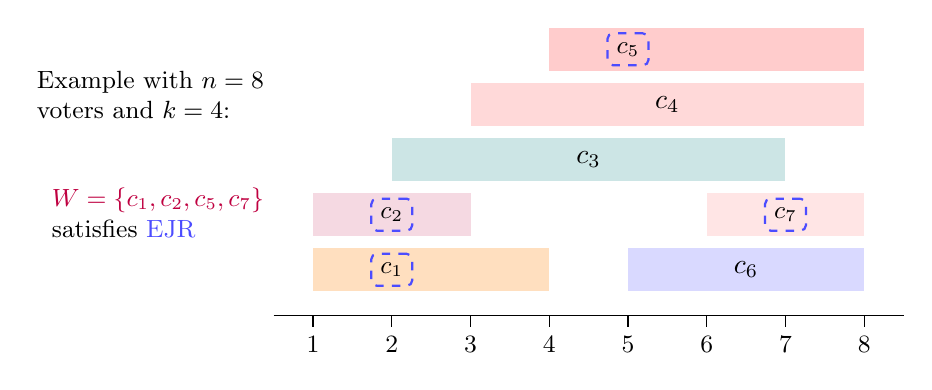
\begin{tikzpicture}[
        bar/.style={minimum height=0.55cm, inner sep=0pt, anchor=west, font=\small},
        inW/.style={draw=blue!70, thick, dashed, rounded corners=2pt, font=\small\bfseries}
    ]

    \def\s{1.0} % scale: 1 unit per voter

    % c1: voters 1--4
    \fill[orange!25] (1*\s, 0) rectangle (4*\s, 0.55);
    \node[inW] at (2*\s, 0.275) {$c_1$};

    % c2: voters 1--3
    \fill[purple!15] (1*\s, 0.7) rectangle (3*\s, 1.25);
    \node[inW] at (2*\s, 0.975) {$c_2$};

    % c3: voters 2--7
    \fill[teal!20] (2*\s, 1.4) rectangle (7*\s, 1.95);
    \node at (4.5*\s, 1.675) {$c_3$};

    % c4: voters 3--8
    \fill[red!15] (3*\s, 2.1) rectangle (8*\s, 2.65);
    \node at (5.5*\s, 2.375) {$c_4$};

    % c5: voters 4--8
    \fill[red!20] (4*\s, 2.8) rectangle (8*\s, 3.35);
    \node[inW] at (5*\s, 3.075) {$c_5$};

    % c6: voters 5--8
    \fill[blue!15] (5*\s, 0) rectangle (8*\s, 0.55);
    \node at (6.5*\s, 0.275) {$c_6$};

    % c7: voters 6--8
    \fill[pink!40] (6*\s, 0.7) rectangle (8*\s, 1.25);
    \node[inW] at (7*\s, 0.975) {$c_7$};

    % Axis
    \draw (0.5*\s, -0.3) -- (8.5*\s, -0.3);
    \foreach \x in {1,...,8} {
        \draw (\x*\s, -0.3) -- (\x*\s, -0.45);
        \node[below, font=\small] at (\x*\s, -0.45) {\x};
    }

    % Label
    \node[anchor=east, align=left, font=\small] at (0.5*\s, 2.5) {
        Example with $n = 8$\\
        voters and $k = 4$:
    };
    \node[anchor=east, align=left, font=\small] at (0.5*\s, 1) {
        {\color{purple} $W = \{c_1, c_2, c_5, c_7\}$}\\
        satisfies \textcolor{blue!70}{EJR}
    };

    \end{tikzpicture}
    \end{center}
\end{example}


\begin{remark}[Finding Proportional Committees Efficiently]
    So far, we have largely talked about verifying a committee satisfies 
    certain properties, but we have not talked about how to find a committee that satisfies these properties.

    \begin{itemize}
        \item A committee satsifying JR can be found efficiently (Exercise: Why?)
        \item PAV satsifies EJR$^+$ (and EJR) but as noted, cannot be computed efficiently
    \end{itemize}
\end{remark}

\begin{theorem}
    A committee satisfying EJR$^+$ can be 
    computed efficiently.
\end{theorem}
\begin{proof}[Sketch]
    Start with an arbritrary committee of appropriate size.
    Iterate over all pairs of candidates where one candidate is in the 
    committee and one is outside of the committee.
    Determine if swapping 
    them would increase the PAV score of the committee, if so we swap them and repeat.
    Eventually, we reach some \emph{PAV-Score local minima}, and then we terminate.

    It turns out, that this local minima must satisfy
    EJR$^+$.
\end{proof}

\begin{remark}
    For several reasons, this doesn't make for a particularly convinving or 
    \emph{principled/nice} voting rules.
    Later, people came up with sequential rules that also 
    satisfy 
    EJR$^+$, and are also polynomial time computable.
\end{remark}

\begin{definition}[Profitable Deviation]
    Given a committee 
    $W$ and a group of voters $S \subseteq N$, a set of candidates $T \subseteq C$ is a 
    \emph{profitable deviation} if
    \[
        |T \cap A_i| > |W \cap A_i| \text{\qquad for all $i \in S$}
    \]
\end{definition}

\begin{definition}[Core Stability]
    A committee $W$ is \emph{core stable}
    if there is no group of voters $S$ and set of candidates $T$ such that
    $|T| \leq |S| \cdot \frac{k}{n}$ and $T$ is a profitable deviation for $S$ from $W$.

    \unclear{Intuition: //TODO}

    The \emph{core} consists of all 
    committees that are core stable.
\end{definition}

\begin{remark}
    It is an open question whether the core is always non-empty.
\end{remark}


\begin{proposition}[EJR's relation to Core Stability]
    Any core stable committee 
    is EJR, that is 
    core stability is 
    a stronger property than EJR.
\end{proposition}
\begin{proof}
    Idea: Show the contrapositive.
    \unclear{TODO}
\end{proof}
\begin{example}
    We may have that 
    a committee is EJR but not core stable.

    For example, with $k=10$, $n=20$ and $C = \set{x_1, \dots, x_{10}, y, z}$, 
    \[
        3 \times \set{x_1, y} \qquad 3 \times \set{x_1, z} 
        \qquad 14 \times \set{x_2, \dots x_{10}}
    \]
    
    $W := \set{x_1, \dots, x_10}$
    satisfies EJR, but the group of voters approving $y$ and $z$ can profitably deviate to $\set{x_1, y, z}$.

    This exemplifies the difference between the notions.
    Core stability considers all possible deviations, whereas 
    EJR only considers deviations restricted to cohesive groups.
\end{example}

\subsection{Approval-based Multiwinner Voting's relation to Apportionment}

\begin{idea}
    The apportionment setting may be viewed as a special case of 
    the approval-based multiwinner voting setting, where
    we partition the candidates into sets 
    $C_1, \dots, C_m$ (where $C_j \geq k$
    \footnote{To ensure that, in principle, each party could fill all 
    seats.}), and each voter $i \in N$, has 
    $A_i = C_j$ for some $j$.

    In this setting, 
    $v_j = |N_j|$ where $N_j = \{i \in N : A_i = C_j\}$, and
    $k = h$.

    Thus, we can see 
    the apportionment setting as a special case of the approval-based multiwinner voting setting, and
    can consider how our 
    approval-based multiwinner rules perform in this setting.
\end{idea}

\begin{example}[Apportionment to Multiwinner Translation]
    \textbf{Step 1:} Translate $(v, h) \longrightarrow (A_N, k)$.

    Given $v = (30, 18, 7)$, $h = 4$. 
    Create $|C_j| = k = 4$ candidates per party:
    \[
        C = \underbrace{\set{a_1, a_2, a_3, a_4}}_{P_1} 
        \cup \underbrace{\set{b_1, b_2, b_3, b_4}}_{P_2} 
        \cup \underbrace{\set{c_1, c_2, c_3, c_4}}_{P_3}
    \]
    Set $k = h = 4$. The approval profile is:
    \begin{center}
    \begin{tabular}{r l}
        $30 \times$ & $\{a_1, a_2, a_3, a_4\}$ \\
        $18 \times$ & $\{b_1, b_2, b_3, b_4\}$ \\
        $7 \times$  & $\{c_1, c_2, c_3, c_4\}$
    \end{tabular}
    \end{center}

    \textbf{Step 2:} Apply rule to $(A_N, k)$:
    say, 
    $W = \{a_1, a_2, a_3, b_1\}$.

    \textbf{Step 3:} Read off seat distribution: 
    $(|W \cap C_1|, |W \cap C_2|, |W \cap C_3|) = (3, 1, 0)$.
\end{example}

\begin{theorem}[$\vec{w}$-PAV induces Divisor methods]
    Let $\vec{w} = (w_1, w_2, \dots)$ be a weight vector with 
    $w_j \geq w_{j+1} > 0$ for all $j \in \mathbb{N}$.
    Then, the apportionment method induced by $w$-PAV coincides with the 
    divisor method based on divisor sequence $d(j) = 1/w_j$.

    \begin{itemize}
        \item PAV (weight vector $w_j = 1/j$) induces the 
        D'Hondt method (divisors $1, 2, 3, \dots$).
        \item $w$-PAV with $w = (1, 1/3, 1/5, \dots)$ induces the 
        Sainte-Lagu\"e method (divisors $1, 3, 5, \dots$).
    \end{itemize}
\end{theorem}

\begin{proposition}
    If an approval-based multiwinner rule satisfies EJR,
    then the apportionment method it induces satisfies the lower quota property.
\end{proposition}

\begin{observation}
    Recall that DHondt's method is the 
    only divisor method satisfying 
    the lower quota property,
    and likewise 
    PAV is the only $\vec{w}$-PAV rule satisfying EJR.
\end{observation}

\unclear{TODO: Crib sheet for all the rules and the properties that they satisfy.}

\bibliographystyle{plain}
\bibliography{refs}


\end{document}